\pdfminorversion=6 % this is needed to be able to include pdf 1.6. 
                    % For some reasons some old HPSG proceedings have pdf 1.6
\documentclass[11pt,a4paper,fleqn]{article}
\usepackage{times}
\thispagestyle{empty}



\usepackage[T1]{fontenc}   % Silbentrennung

\usepackage[utf8x]{inputenc}
                                                                                                                             
\hyphenation{Acad-e-my}

\usepackage[bookmarks=true,bookmarksopen=true,%
breaklinks=true,%
draft=false,plainpages=false,hyperfootnotes=false,%
pdfauthor={Stefan Müller (Editor)},%
pdftitle={Proceedings of the 16th International Conference on Head-Driven Phrase Structure Grammar},%
pdfkeywords={HPSG}%,
pdftex=true%
%ps2pdf=true  %ohne diesen Treiber geht der Zeilenumbruch in URLs
]{hyperref}% for pdf files
\hypersetup{colorlinks=false, pdfborder={0 0 0}}

\usepackage{pdfpages}
\pdfinclusioncopyfonts=1

\newcommand\formatauthor[2]{\begin{tabular}[t]{@{}c@{}}
  {\LARGE#1\strut}\\
  {\small#2\strut}\\
  \rule{\dimexpr0.5\linewidth-1em}{0pt}
  \end{tabular}\xhfill\ignorespaces}
\newcommand\xhfill{\hspace{1em plus 1fill}}

\begin{document}

\begin{center}
{\Large
                {\bfseries Proceedings of the 16th International Conference on\par Head-Driven Phrase Structure Grammar\par}

                \vspace{8ex}

                     Georg-August-Universit\"{a}t G{\"o}ttingen, Germany\\[\baselineskip]

                        Stefan M{\"u}ller (Editor)\\[\baselineskip]

                                2009\\[\baselineskip]

                          CSLI Publications\\[\baselineskip]

              http://csli-publications.stanford.edu/HPSG/2009 \\[4\baselineskip]

The papers are published under a \href{http://creativecommons.org/licenses/by/4.0/}{CC-BY license}:\\[3pt]
\href{http://creativecommons.org/licenses/by/4.0/}{http://creativecommons.org/licenses/by/4.0/}
}
\end{center}
\newpage
\tableofcontents

\newpage

\section{Editor's Note}
%% -*- coding:utf-8 -*-
The 16th International Conference on Head-Driven Phrase Structure Grammar (2009) was held in Göttingen.

The conference featured 2 invited talks and 19 papers selected by the program committee (Anne
Abeille, Doug Arnold [chair], Olivier Bonami, Bob Borsley, Gosse Bouma, Rui Chaves, Berthold
Crysmann, Markus Egg, Elisabet Engdahl, Dan Flickinger, Jonathan Ginzburg, Chikara Hashimoto,
Jong-Bok Kim, Tibor Kiss, Anna Kupsc, Shalom Lappin, Bob Levine, Rob Malouf, Detmar Meurers, Stefan
Müller, Tsuneko Nakazawa, Gerald Penn, Adam Przepiorkowski, Frank Richter, Louisa Sadler, Ivan Sag,
Jesse Tseng, Stephen Wechsler).


In total there were 34  submissions to the conference.
We want to thank the  program committee for putting this nice program together.



Thanks go to Anke Holler, Manfred Sailer, Heike Walker, Gert Webelhuth [chair], who were in charge of local arrangements.


As in the past years the contributions to the conference proceedings are based on the five page abstract
that was reviewed by the respective program committees, but there is no additional reviewing of the
longer contribution to the proceedings.
To ensure easy access and fast publication we have chosen an electronic format.


The proceedings include all the papers except those by Danièle Godard and Anne Abeillé and Polly Jacobson.

\newpage
        \setcounter{page}{5}
        \phantomsection
        \addcontentsline{toc}{section}{Gabriela Bîlbîie, Fr{\'e}d{\'e}ric Laurens: A Construction-based Analysis of Verbless Relative Adjuncts in French and Romanian}
\thispagestyle{empty}

\begin{center}
  {\huge\bfseries A Construction-based Analysis of Verbless Relative Adjuncts in French and Romanian\par}

  \bigskip

~\\
\begingroup
\setlength{\leftskip}{0pt plus 1fill}
\setlength{\rightskip}{0pt plus 1fill}
\setlength{\parindent}{0pt}
\setlength{\parfillskip}{0pt}
  \formatauthor{Gabriela Bîlbîie}{\begin{tabular}{@{}c@{}}LLF, Université Paris Diderot Paris 7\end{tabular}}
\formatauthor{Frédéric Laurens}{\begin{tabular}{@{}c@{}}LLF, Université Paris Diderot Paris 7\end{tabular}}

\par\endgroup

  \vspace*{8ex}

  Proceedings of the 16th International Conference on\par Head-Driven Phrase Structure Grammar

  \bigskip

  Georg-August-Universit\"{a}t G{\"o}ttingen, Germany

  \medskip

  Stefan Müller (Editor)

  \medskip

  2009

  \medskip

  CSLI Publications

  \medskip

  pages 5--25

  \medskip

  \url{http://csli-publications.stanford.edu/HPSG/2009}
\end{center}
\vfill

\noindent



\vfill
\noindent
% APA Style
Bîlbîie, Gabriela, \& Laurens, Frédéric. 2009. A Construction-based Analysis of Verbless Relative Adjuncts in French and Romanian. In Müller, Stefan (Ed.), \emph{{Proceedings of the 16th International Conference on Head-Driven Phrase Structure Grammar, Georg-August-Universit\"{a}t G{\"o}ttingen, Germany}}, 5--25. Stanford,
CA: CSLI Publications. \hfill\href{http://creativecommons.org/licenses/by/4.0/}{\includegraphics[height=.75em]{Includes/ccby.eps}}

\newpage
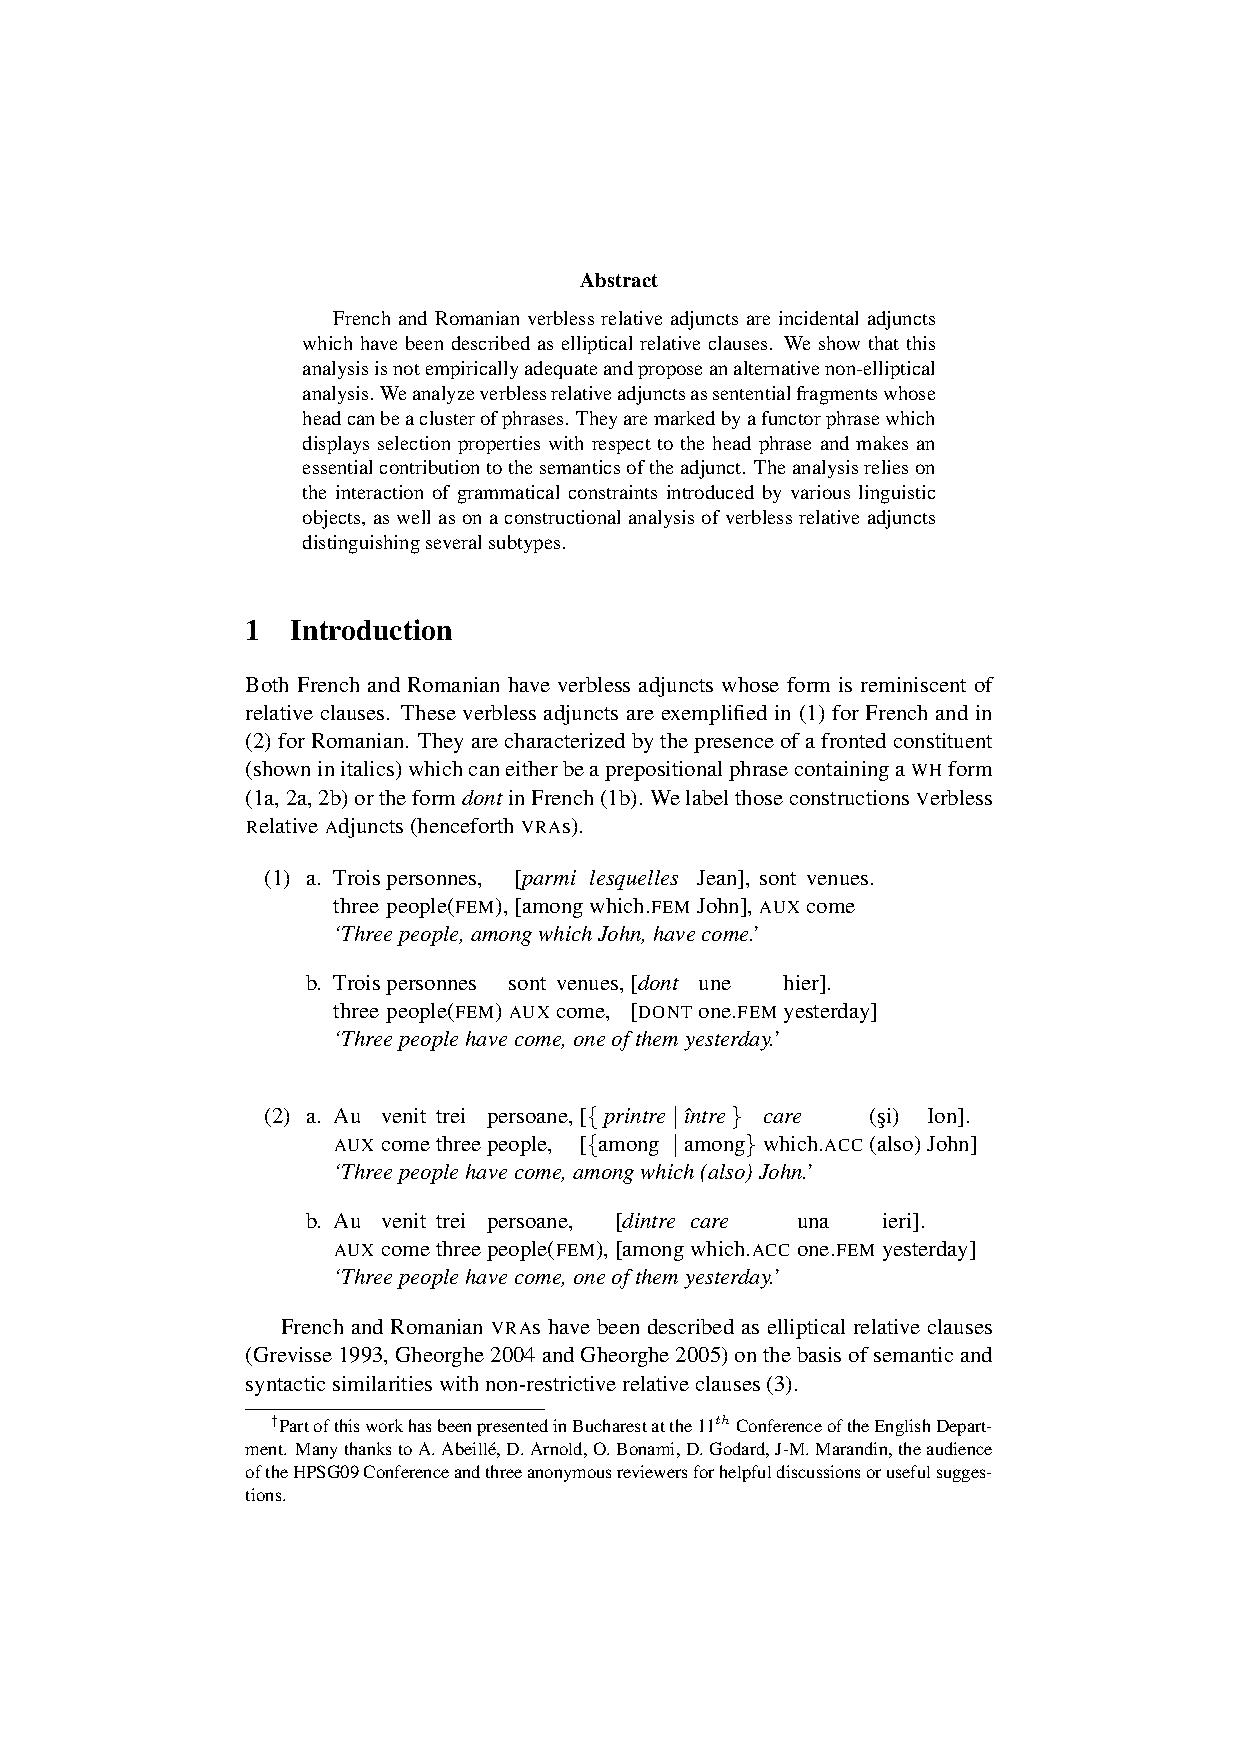
\includepdf[pages=-,pagecommand=\thispagestyle{plain}]{Includes/bilbiie-laurens.pdf}
        \setcounter{page}{26}
        \phantomsection
        \addcontentsline{toc}{section}{Olivier Bonami, Pollet Samvelian: Inflectional periphrasis in Persian}
\thispagestyle{empty}

\begin{center}
  {\huge\bfseries Inflectional periphrasis in Persian\par}

  \bigskip

~\\
\begingroup
\setlength{\leftskip}{0pt plus 1fill}
\setlength{\rightskip}{0pt plus 1fill}
\setlength{\parindent}{0pt}
\setlength{\parfillskip}{0pt}
  \formatauthor{Olivier Bonami}{\begin{tabular}{@{}c@{}}Université Paris-Sorbonne and Laboratoire de Linguistique Formelle\end{tabular}}
\formatauthor{Pollet Samvelian}{\begin{tabular}{@{}c@{}}Université Paris 3 Sorbonne nouvelle and Mondes iranien et indien\end{tabular}}

\par\endgroup

  \vspace*{8ex}

  Proceedings of the 16th International Conference on\par Head-Driven Phrase Structure Grammar

  \bigskip

  Georg-August-Universit\"{a}t G{\"o}ttingen, Germany

  \medskip

  Stefan Müller (Editor)

  \medskip

  2009

  \medskip

  CSLI Publications

  \medskip

  pages 26--46

  \medskip

  \url{http://csli-publications.stanford.edu/HPSG/2009}
\end{center}
\vfill

\noindent



\vfill
\noindent
% APA Style
Bonami, Olivier, \& Samvelian, Pollet. 2009. Inflectional periphrasis in Persian. In Müller, Stefan (Ed.), \emph{{Proceedings of the 16th International Conference on Head-Driven Phrase Structure Grammar, Georg-August-Universit\"{a}t G{\"o}ttingen, Germany}}, 26--46. Stanford,
CA: CSLI Publications. \hfill\href{http://creativecommons.org/licenses/by/4.0/}{\includegraphics[height=.75em]{Includes/ccby.eps}}

\newpage
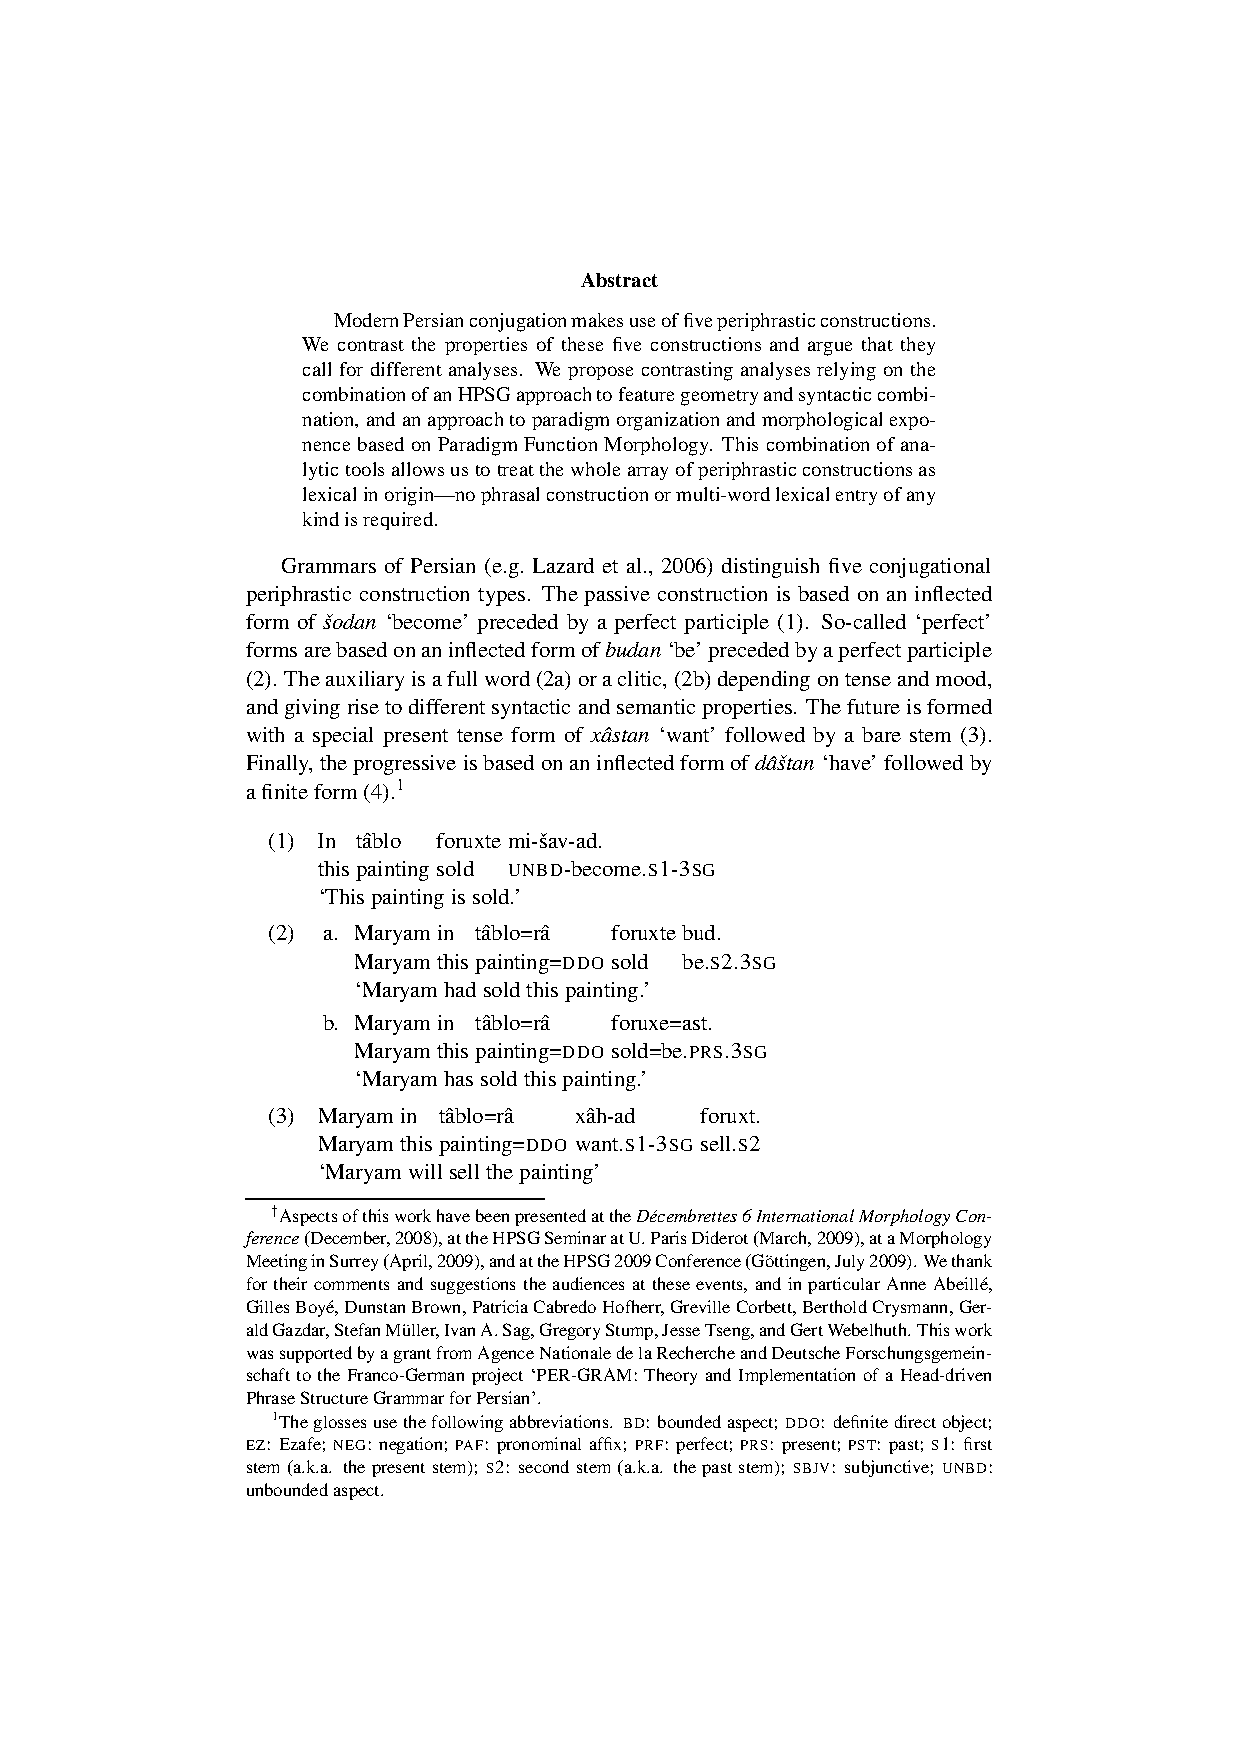
\includepdf[pages=-,pagecommand=\thispagestyle{plain}]{Includes/bonami-samvelian.pdf}
        \setcounter{page}{47}
        \phantomsection
        \addcontentsline{toc}{section}{Rui P. Chaves: Construction-based Cumulation and Adjunct Extraction}
\thispagestyle{empty}

\begin{center}
  {\huge\bfseries Construction-based Cumulation and Adjunct Extraction\par}

  \bigskip

~\\
\begingroup
\setlength{\leftskip}{0pt plus 1fill}
\setlength{\rightskip}{0pt plus 1fill}
\setlength{\parindent}{0pt}
\setlength{\parfillskip}{0pt}
  \formatauthor{Rui P. Chaves}{\begin{tabular}{@{}c@{}}University at Buffalo, SUNY\end{tabular}}

\par\endgroup

  \vspace*{8ex}

  Proceedings of the 16th International Conference on\par Head-Driven Phrase Structure Grammar

  \bigskip

  Georg-August-Universit\"{a}t G{\"o}ttingen, Germany

  \medskip

  Stefan Müller (Editor)

  \medskip

  2009

  \medskip

  CSLI Publications

  \medskip

  pages 47--67

  \medskip

  \url{http://csli-publications.stanford.edu/HPSG/2009}
\end{center}
\vfill

\noindent



\vfill
\noindent
% APA Style
Chaves, Rui P. 2009. Construction-based Cumulation and Adjunct Extraction. In Müller, Stefan (Ed.), \emph{{Proceedings of the 16th International Conference on Head-Driven Phrase Structure Grammar, Georg-August-Universit\"{a}t G{\"o}ttingen, Germany}}, 47--67. Stanford,
CA: CSLI Publications. \hfill\href{http://creativecommons.org/licenses/by/4.0/}{\includegraphics[height=.75em]{Includes/ccby.eps}}

\newpage
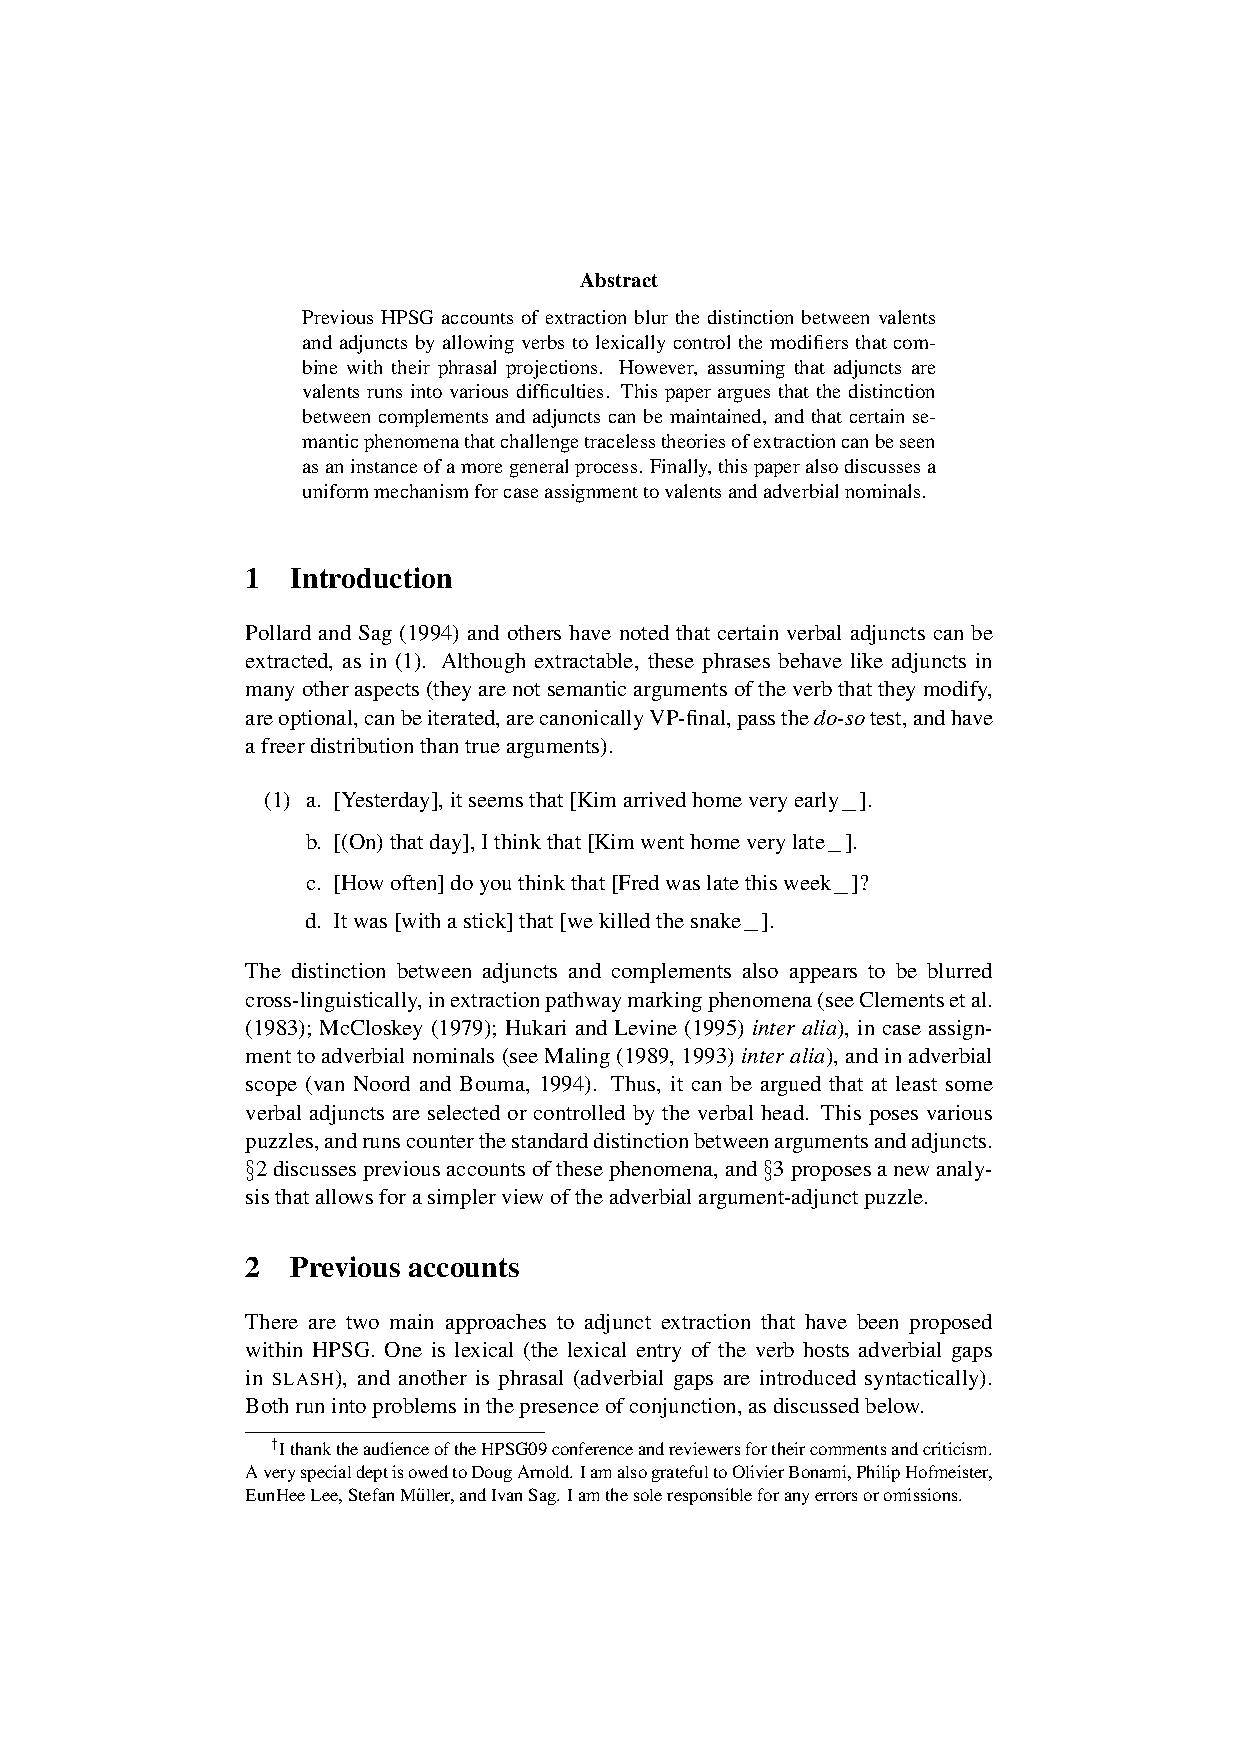
\includepdf[pages=-,pagecommand=\thispagestyle{plain}]{Includes/chaves.pdf}
        \setcounter{page}{68}
        \phantomsection
        \addcontentsline{toc}{section}{Berthold Crysmann: Deriving Superficial Ergativity in Nias}
\thispagestyle{empty}

\begin{center}
  {\huge\bfseries Deriving Superficial Ergativity in Nias\par}

  \bigskip

~\\
\begingroup
\setlength{\leftskip}{0pt plus 1fill}
\setlength{\rightskip}{0pt plus 1fill}
\setlength{\parindent}{0pt}
\setlength{\parfillskip}{0pt}
  \formatauthor{Berthold Crysmann}{\begin{tabular}{@{}c@{}}Universität Bonn and Universität des Saarlandes\end{tabular}}

\par\endgroup

  \vspace*{8ex}

  Proceedings of the 16th International Conference on\par Head-Driven Phrase Structure Grammar

  \bigskip

  Georg-August-Universit\"{a}t G{\"o}ttingen, Germany

  \medskip

  Stefan Müller (Editor)

  \medskip

  2009

  \medskip

  CSLI Publications

  \medskip

  pages 68--88

  \medskip

  \url{http://csli-publications.stanford.edu/HPSG/2009}
\end{center}
\vfill

\noindent



\vfill
\noindent
% APA Style
Crysmann, Berthold. 2009. Deriving Superficial Ergativity in Nias. In Müller, Stefan (Ed.), \emph{{Proceedings of the 16th International Conference on Head-Driven Phrase Structure Grammar, Georg-August-Universit\"{a}t G{\"o}ttingen, Germany}}, 68--88. Stanford,
CA: CSLI Publications. \hfill\href{http://creativecommons.org/licenses/by/4.0/}{\includegraphics[height=.75em]{Includes/ccby.eps}}

\newpage
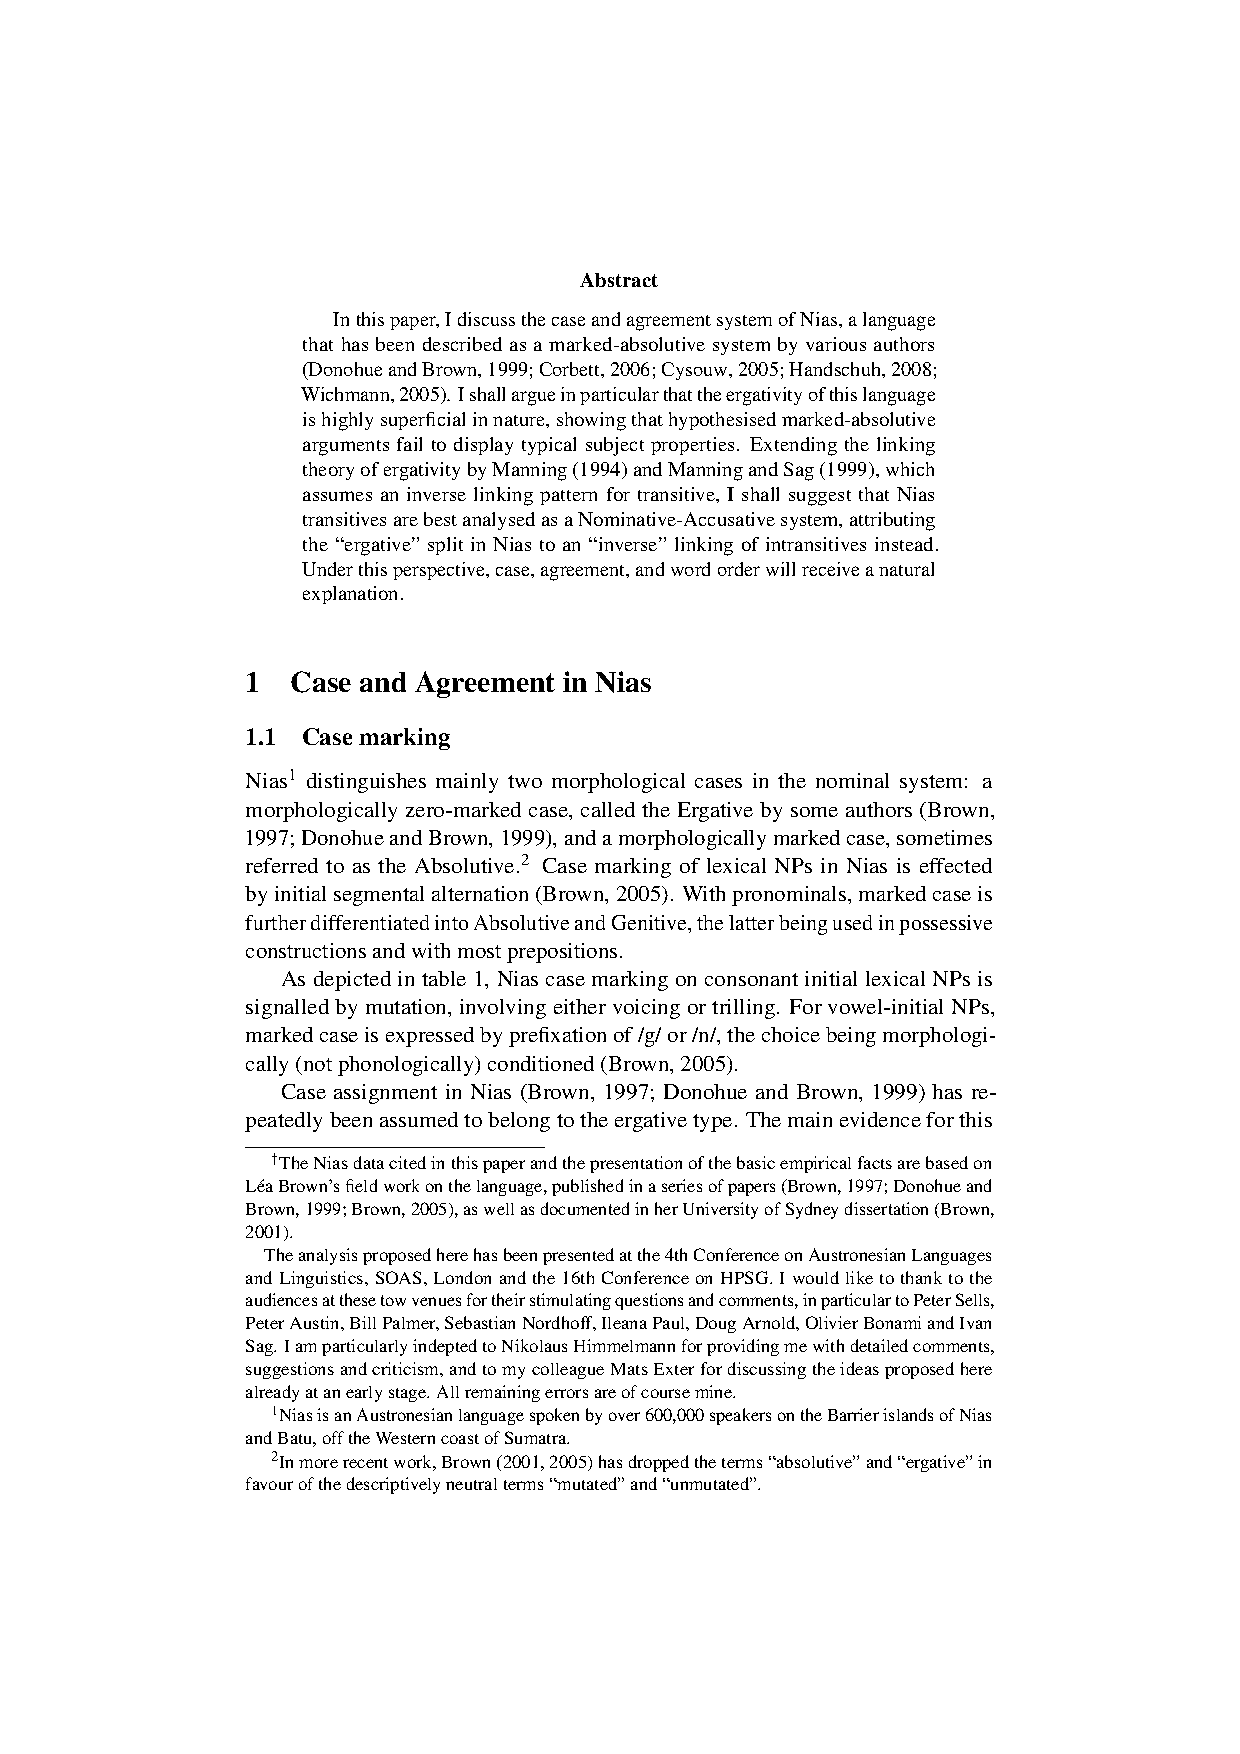
\includepdf[pages=-,pagecommand=\thispagestyle{plain}]{Includes/crysmann.pdf}
        \setcounter{page}{89}
        \phantomsection
        \addcontentsline{toc}{section}{Marianne Desmets, Florence Villoing: French VN lexemes: morphological compounding in HPSG}
\thispagestyle{empty}

\begin{center}
  {\huge\bfseries French VN lexemes: morphological compounding in HPSG\par}

  \bigskip

~\\
\begingroup
\setlength{\leftskip}{0pt plus 1fill}
\setlength{\rightskip}{0pt plus 1fill}
\setlength{\parindent}{0pt}
\setlength{\parfillskip}{0pt}
  \formatauthor{Marianne Desmets}{\begin{tabular}{@{}c@{}}Université Paris Ouest/LLF\end{tabular}}
\formatauthor{Florence Villoing}{\begin{tabular}{@{}c@{}}Université Paris Saint-Denis/SFL\end{tabular}}

\par\endgroup

  \vspace*{8ex}

  Proceedings of the 16th International Conference on\par Head-Driven Phrase Structure Grammar

  \bigskip

  Georg-August-Universit\"{a}t G{\"o}ttingen, Germany

  \medskip

  Stefan Müller (Editor)

  \medskip

  2009

  \medskip

  CSLI Publications

  \medskip

  pages 89--109

  \medskip

  \url{http://csli-publications.stanford.edu/HPSG/2009}
\end{center}
\vfill

\noindent



\vfill
\noindent
% APA Style
Desmets, Marianne, \& Villoing, Florence. 2009. French VN lexemes: morphological compounding in HPSG. In Müller, Stefan (Ed.), \emph{{Proceedings of the 16th International Conference on Head-Driven Phrase Structure Grammar, Georg-August-Universit\"{a}t G{\"o}ttingen, Germany}}, 89--109. Stanford,
CA: CSLI Publications. \hfill\href{http://creativecommons.org/licenses/by/4.0/}{\includegraphics[height=.75em]{Includes/ccby.eps}}

\newpage
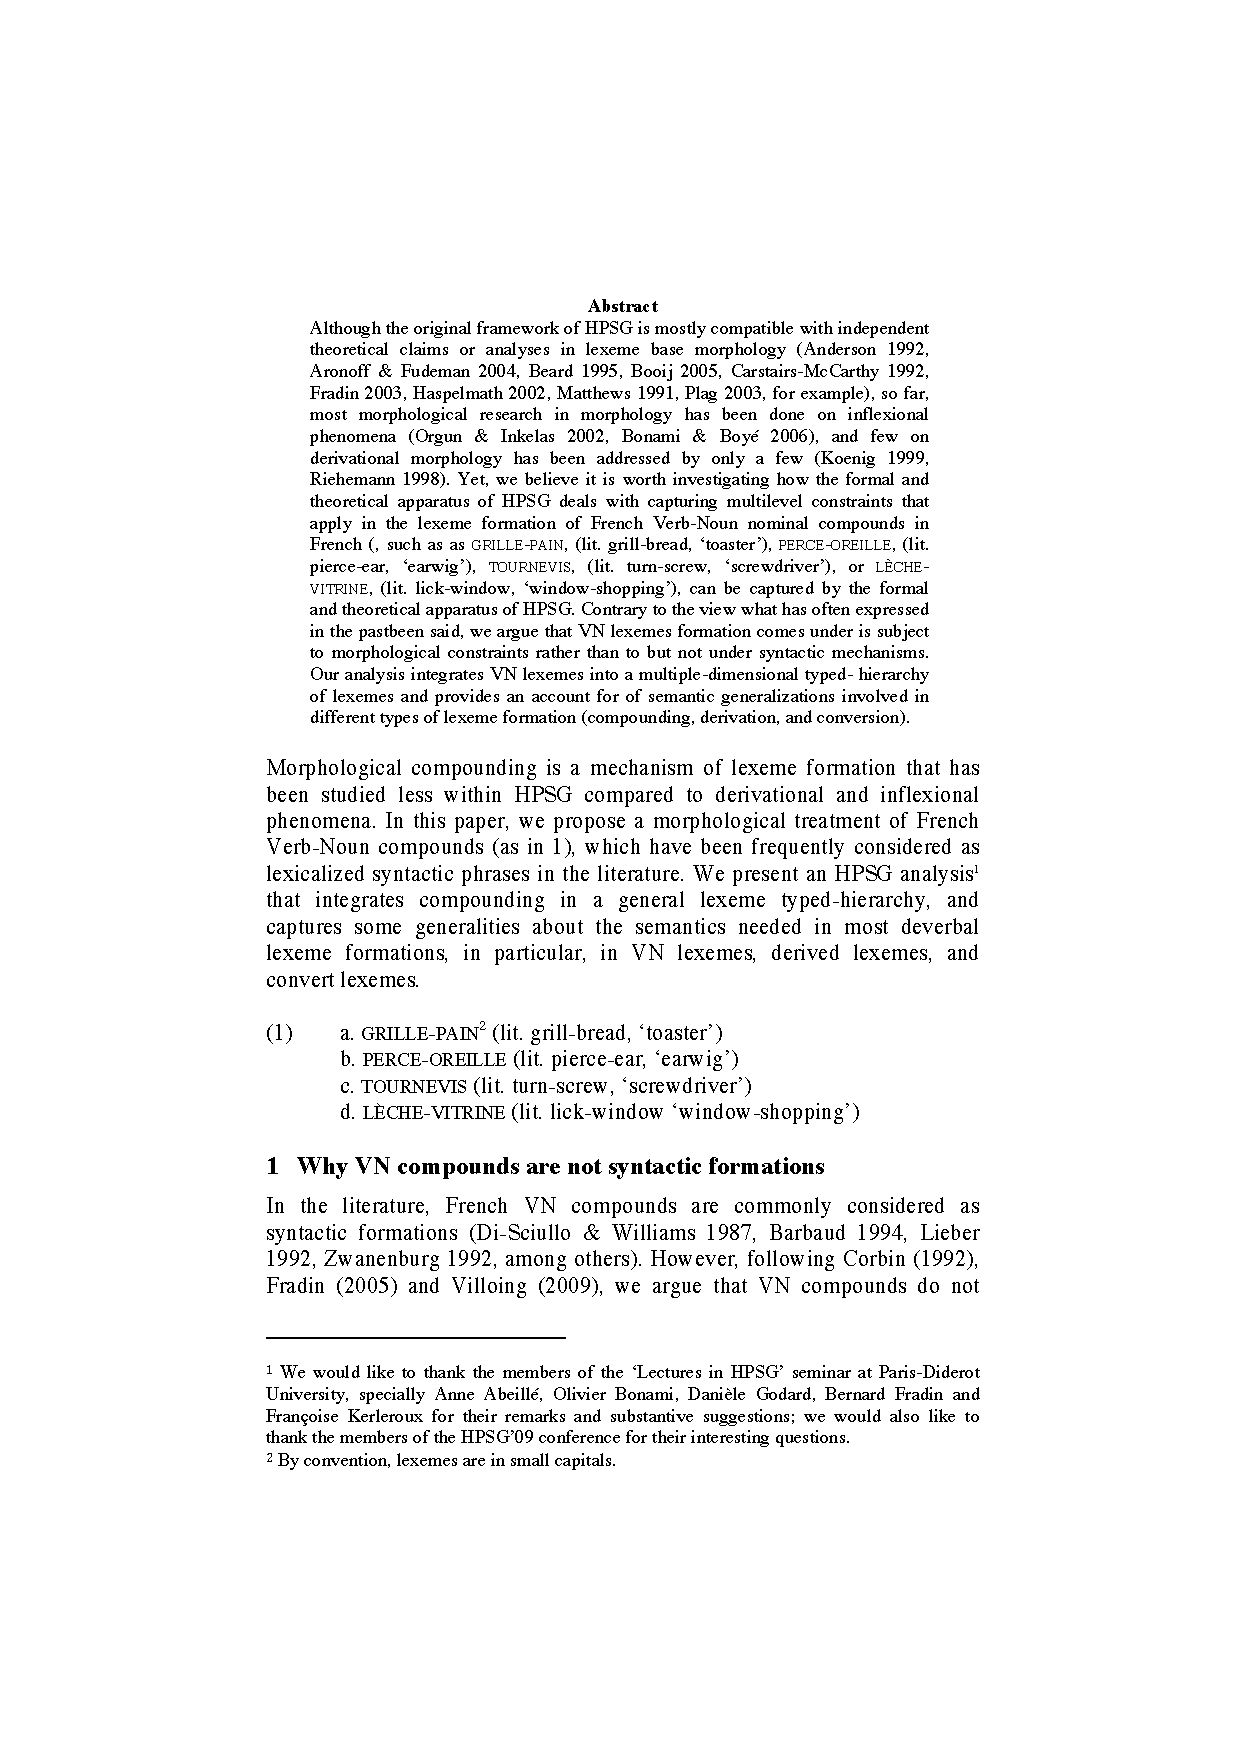
\includepdf[pages=-,pagecommand=\thispagestyle{plain}]{Includes/desmets-villoing.pdf}
        \setcounter{page}{110}
        \phantomsection
        \addcontentsline{toc}{section}{Antske Fokkens, Laurie Poulson, Emily M. Bender: Inflectional Morphology in Turkish VP Coordination}
\thispagestyle{empty}

\begin{center}
  {\huge\bfseries Inflectional Morphology in Turkish VP Coordination\par}

  \bigskip

~\\
\begingroup
\setlength{\leftskip}{0pt plus 1fill}
\setlength{\rightskip}{0pt plus 1fill}
\setlength{\parindent}{0pt}
\setlength{\parfillskip}{0pt}
  \formatauthor{Antske Fokkens}{\begin{tabular}{@{}c@{}}Universität des Saarlandes\end{tabular}}
\formatauthor{Laurie Poulson}{\begin{tabular}{@{}c@{}}University of Washington\end{tabular}}
\formatauthor{Emily M. Bender}{\begin{tabular}{@{}c@{}}\end{tabular}}

\par\endgroup

  \vspace*{8ex}

  Proceedings of the 16th International Conference on\par Head-Driven Phrase Structure Grammar

  \bigskip

  Georg-August-Universit\"{a}t G{\"o}ttingen, Germany

  \medskip

  Stefan Müller (Editor)

  \medskip

  2009

  \medskip

  CSLI Publications

  \medskip

  pages 110--130

  \medskip

  \url{http://csli-publications.stanford.edu/HPSG/2009}
\end{center}
\vfill

\noindent



\vfill
\noindent
% APA Style
Fokkens, Antske, Poulson, Laurie, \& Bender, Emily M. 2009. Inflectional Morphology in Turkish VP Coordination. In Müller, Stefan (Ed.), \emph{{Proceedings of the 16th International Conference on Head-Driven Phrase Structure Grammar, Georg-August-Universit\"{a}t G{\"o}ttingen, Germany}}, 110--130. Stanford,
CA: CSLI Publications. \hfill\href{http://creativecommons.org/licenses/by/4.0/}{\includegraphics[height=.75em]{Includes/ccby.eps}}

\newpage
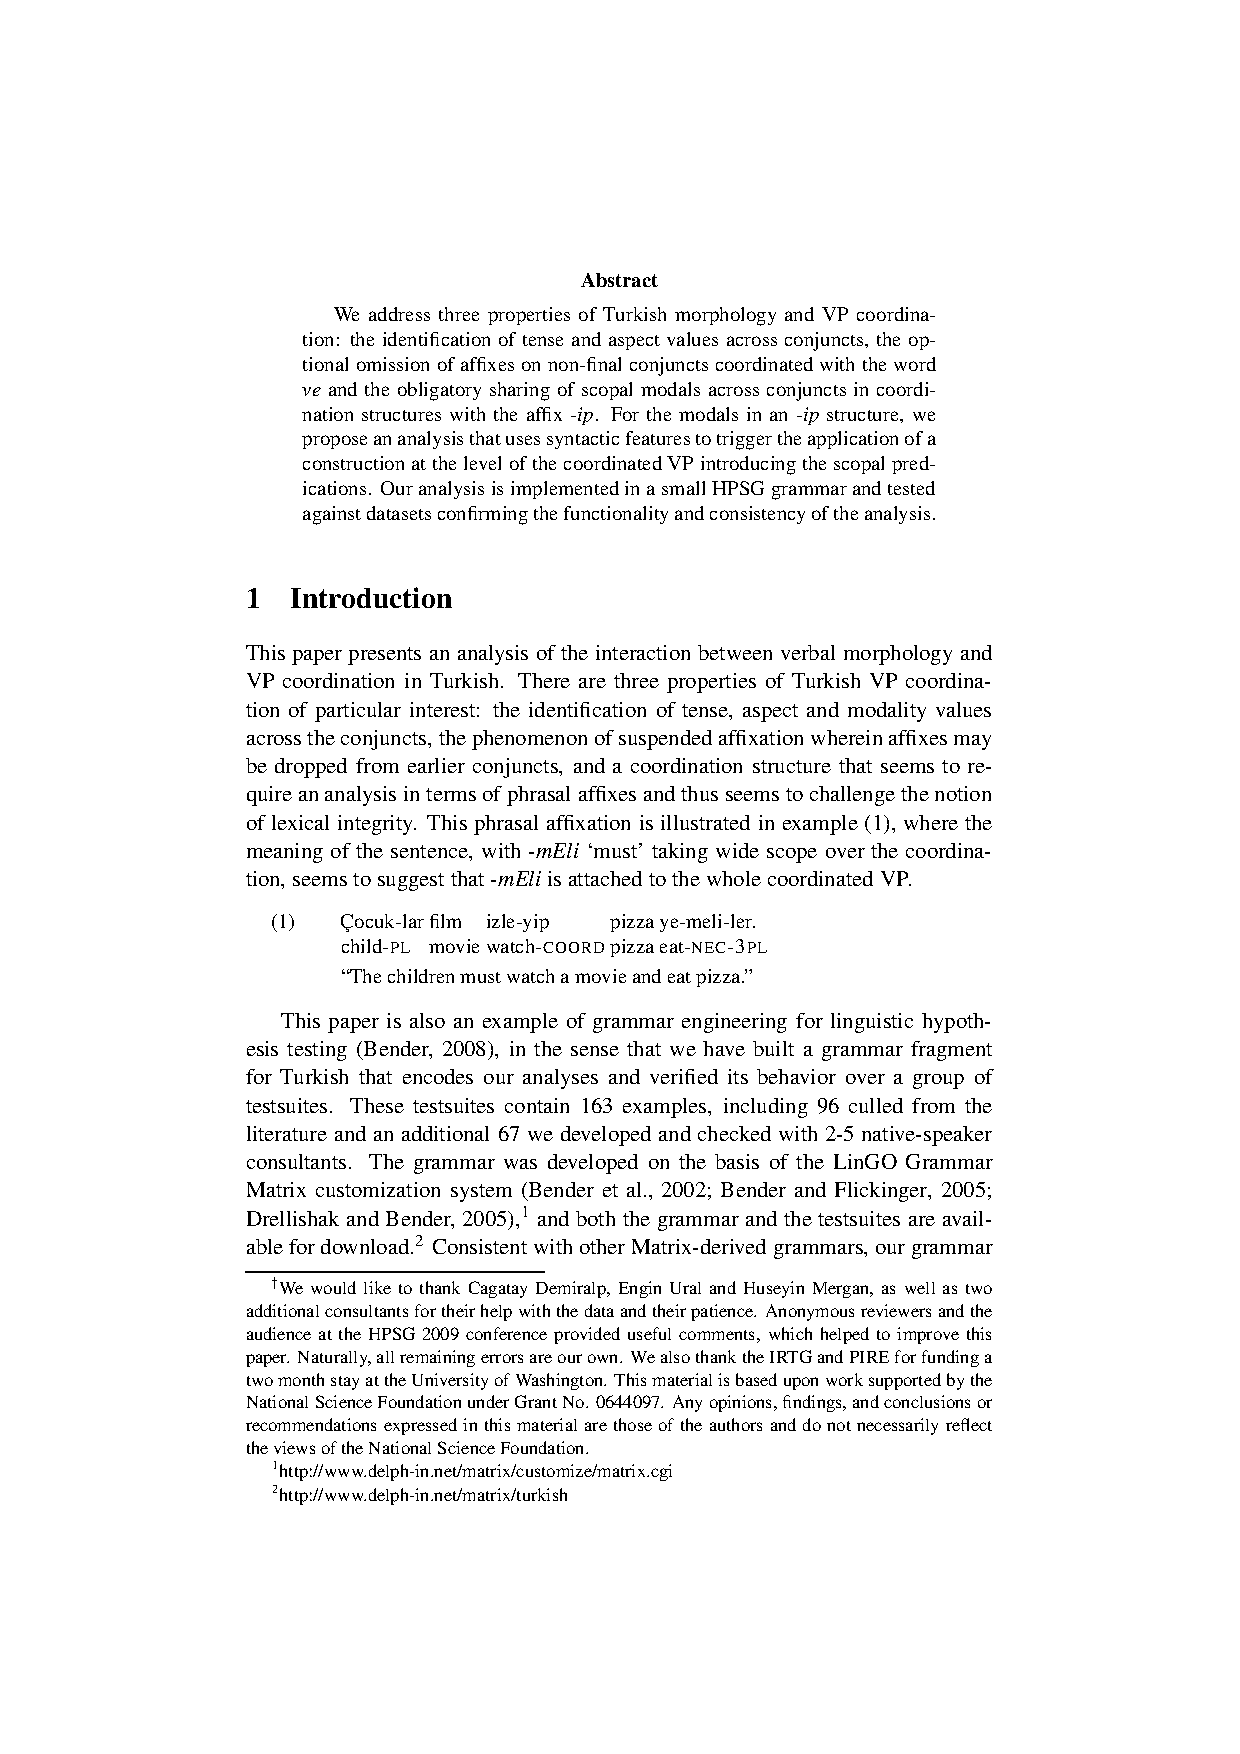
\includepdf[pages=-,pagecommand=\thispagestyle{plain}]{Includes/fpb.pdf}
        \setcounter{page}{131}
        \phantomsection
        \addcontentsline{toc}{section}{Anke Holler: Towards an analysis of the adverbial use of German interrogative \emph{was}
(`what')}
\thispagestyle{empty}

\begin{center}
  {\huge\bfseries Towards an analysis of the adverbial use of German interrogative \emph{was}
(`what')\par}

  \bigskip

~\\
\begingroup
\setlength{\leftskip}{0pt plus 1fill}
\setlength{\rightskip}{0pt plus 1fill}
\setlength{\parindent}{0pt}
\setlength{\parfillskip}{0pt}
  \formatauthor{Anke Holler}{\begin{tabular}{@{}c@{}}University of Göttingen\end{tabular}}

\par\endgroup

  \vspace*{8ex}

  Proceedings of the 16th International Conference on\par Head-Driven Phrase Structure Grammar

  \bigskip

  Georg-August-Universit\"{a}t G{\"o}ttingen, Germany

  \medskip

  Stefan Müller (Editor)

  \medskip

  2009

  \medskip

  CSLI Publications

  \medskip

  pages 131--149

  \medskip

  \url{http://csli-publications.stanford.edu/HPSG/2009}
\end{center}
\vfill

\noindent



\vfill
\noindent
% APA Style
Holler, Anke. 2009. Towards an analysis of the adverbial use of German interrogative \emph{was}
(`what'). In Müller, Stefan (Ed.), \emph{{Proceedings of the 16th International Conference on Head-Driven Phrase Structure Grammar, Georg-August-Universit\"{a}t G{\"o}ttingen, Germany}}, 131--149. Stanford,
CA: CSLI Publications. \hfill\href{http://creativecommons.org/licenses/by/4.0/}{\includegraphics[height=.75em]{Includes/ccby.eps}}

\newpage
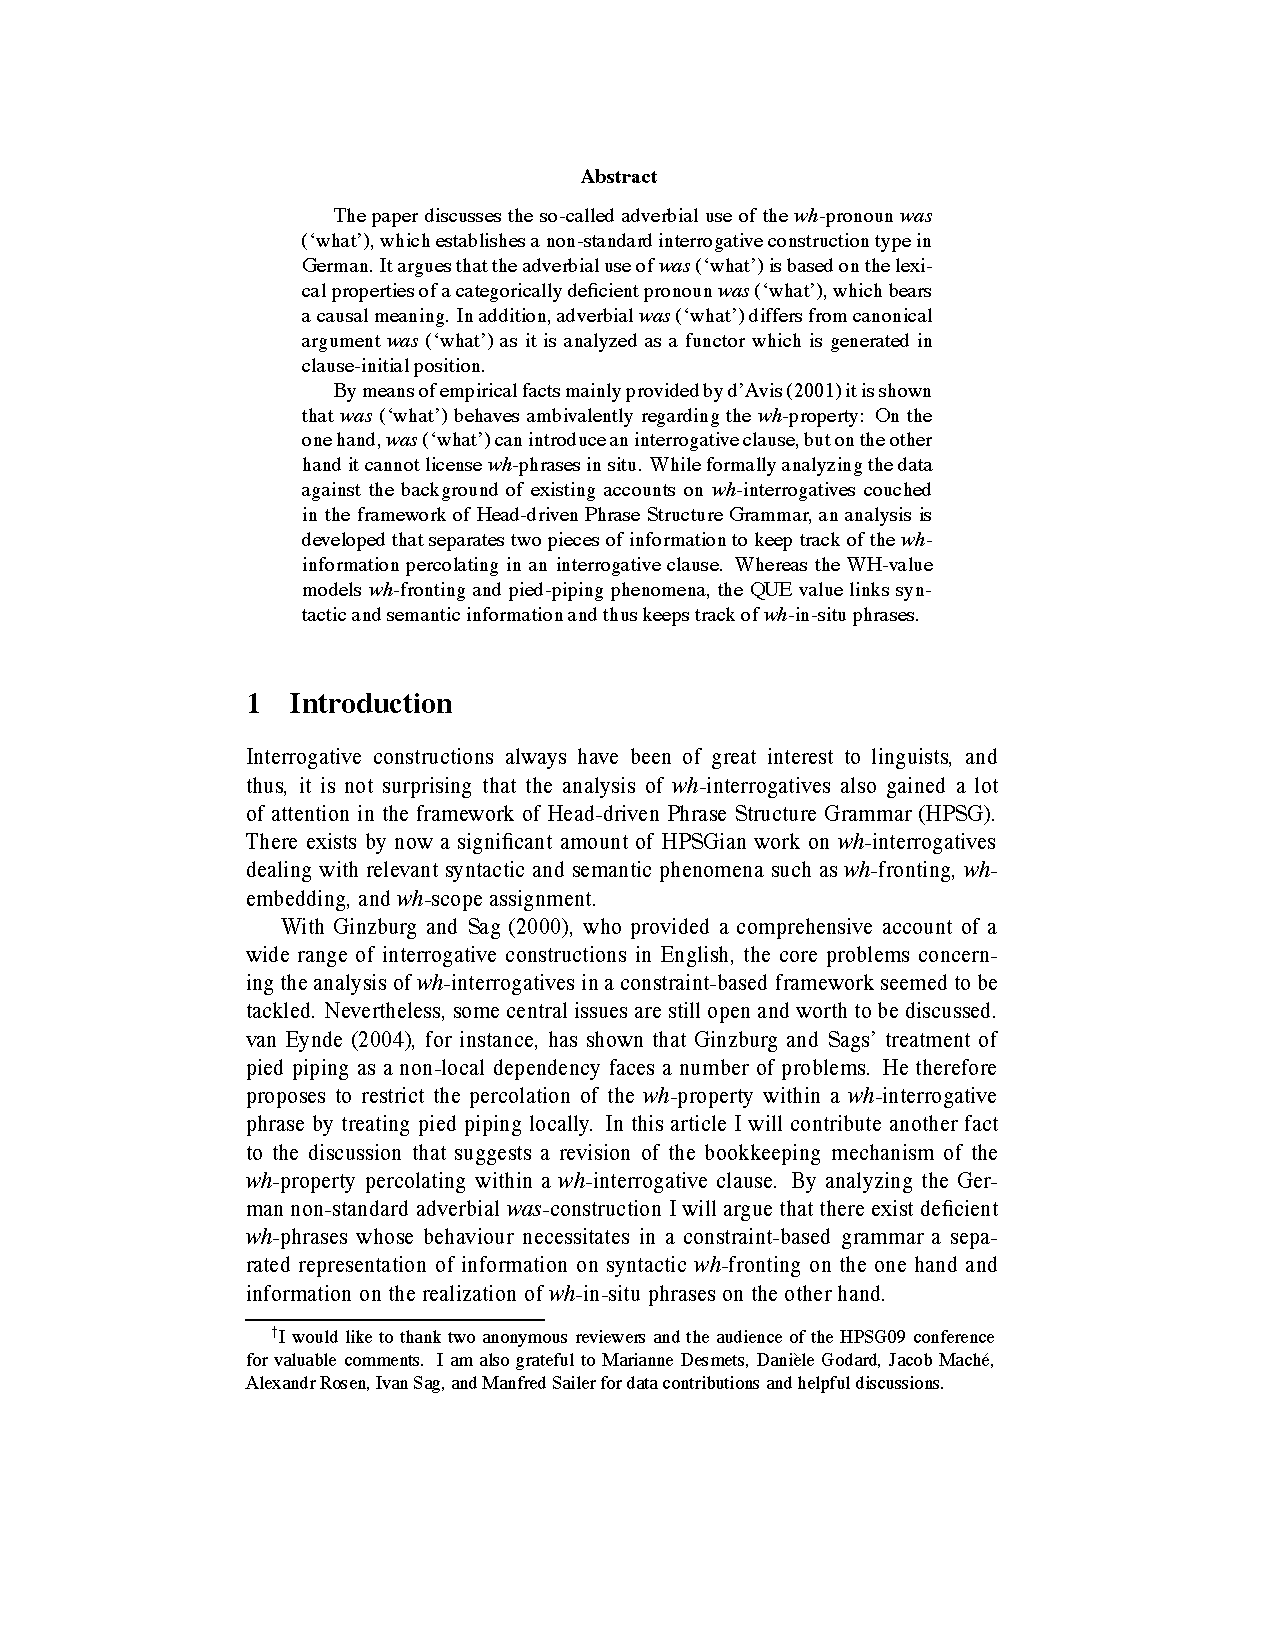
\includepdf[pages=-,pagecommand=\thispagestyle{plain}]{Includes/holler.pdf}
        \setcounter{page}{150}
        \phantomsection
        \addcontentsline{toc}{section}{Gianina Iord\u{a}chioaia, Frank Richter: Negative Concord in Romanian as Polyadic Quantification}
\thispagestyle{empty}

\begin{center}
  {\huge\bfseries Negative Concord in Romanian as Polyadic Quantification\par}

  \bigskip

~\\
\begingroup
\setlength{\leftskip}{0pt plus 1fill}
\setlength{\rightskip}{0pt plus 1fill}
\setlength{\parindent}{0pt}
\setlength{\parfillskip}{0pt}
  \formatauthor{Gianina Iordăchioaia}{\begin{tabular}{@{}c@{}}Universität Stuttgart\end{tabular}}
\formatauthor{Frank Richter}{\begin{tabular}{@{}c@{}}Universität Tübingen\end{tabular}}

\par\endgroup

  \vspace*{8ex}

  Proceedings of the 16th International Conference on\par Head-Driven Phrase Structure Grammar

  \bigskip

  Georg-August-Universit\"{a}t G{\"o}ttingen, Germany

  \medskip

  Stefan Müller (Editor)

  \medskip

  2009

  \medskip

  CSLI Publications

  \medskip

  pages 150--170

  \medskip

  \url{http://csli-publications.stanford.edu/HPSG/2009}
\end{center}
\vfill

\noindent



\vfill
\noindent
% APA Style
Iordăchioaia, Gianina, \& Richter, Frank. 2009. Negative Concord in Romanian as Polyadic Quantification. In Müller, Stefan (Ed.), \emph{{Proceedings of the 16th International Conference on Head-Driven Phrase Structure Grammar, Georg-August-Universit\"{a}t G{\"o}ttingen, Germany}}, 150--170. Stanford,
CA: CSLI Publications. \hfill\href{http://creativecommons.org/licenses/by/4.0/}{\includegraphics[height=.75em]{Includes/ccby.eps}}

\newpage
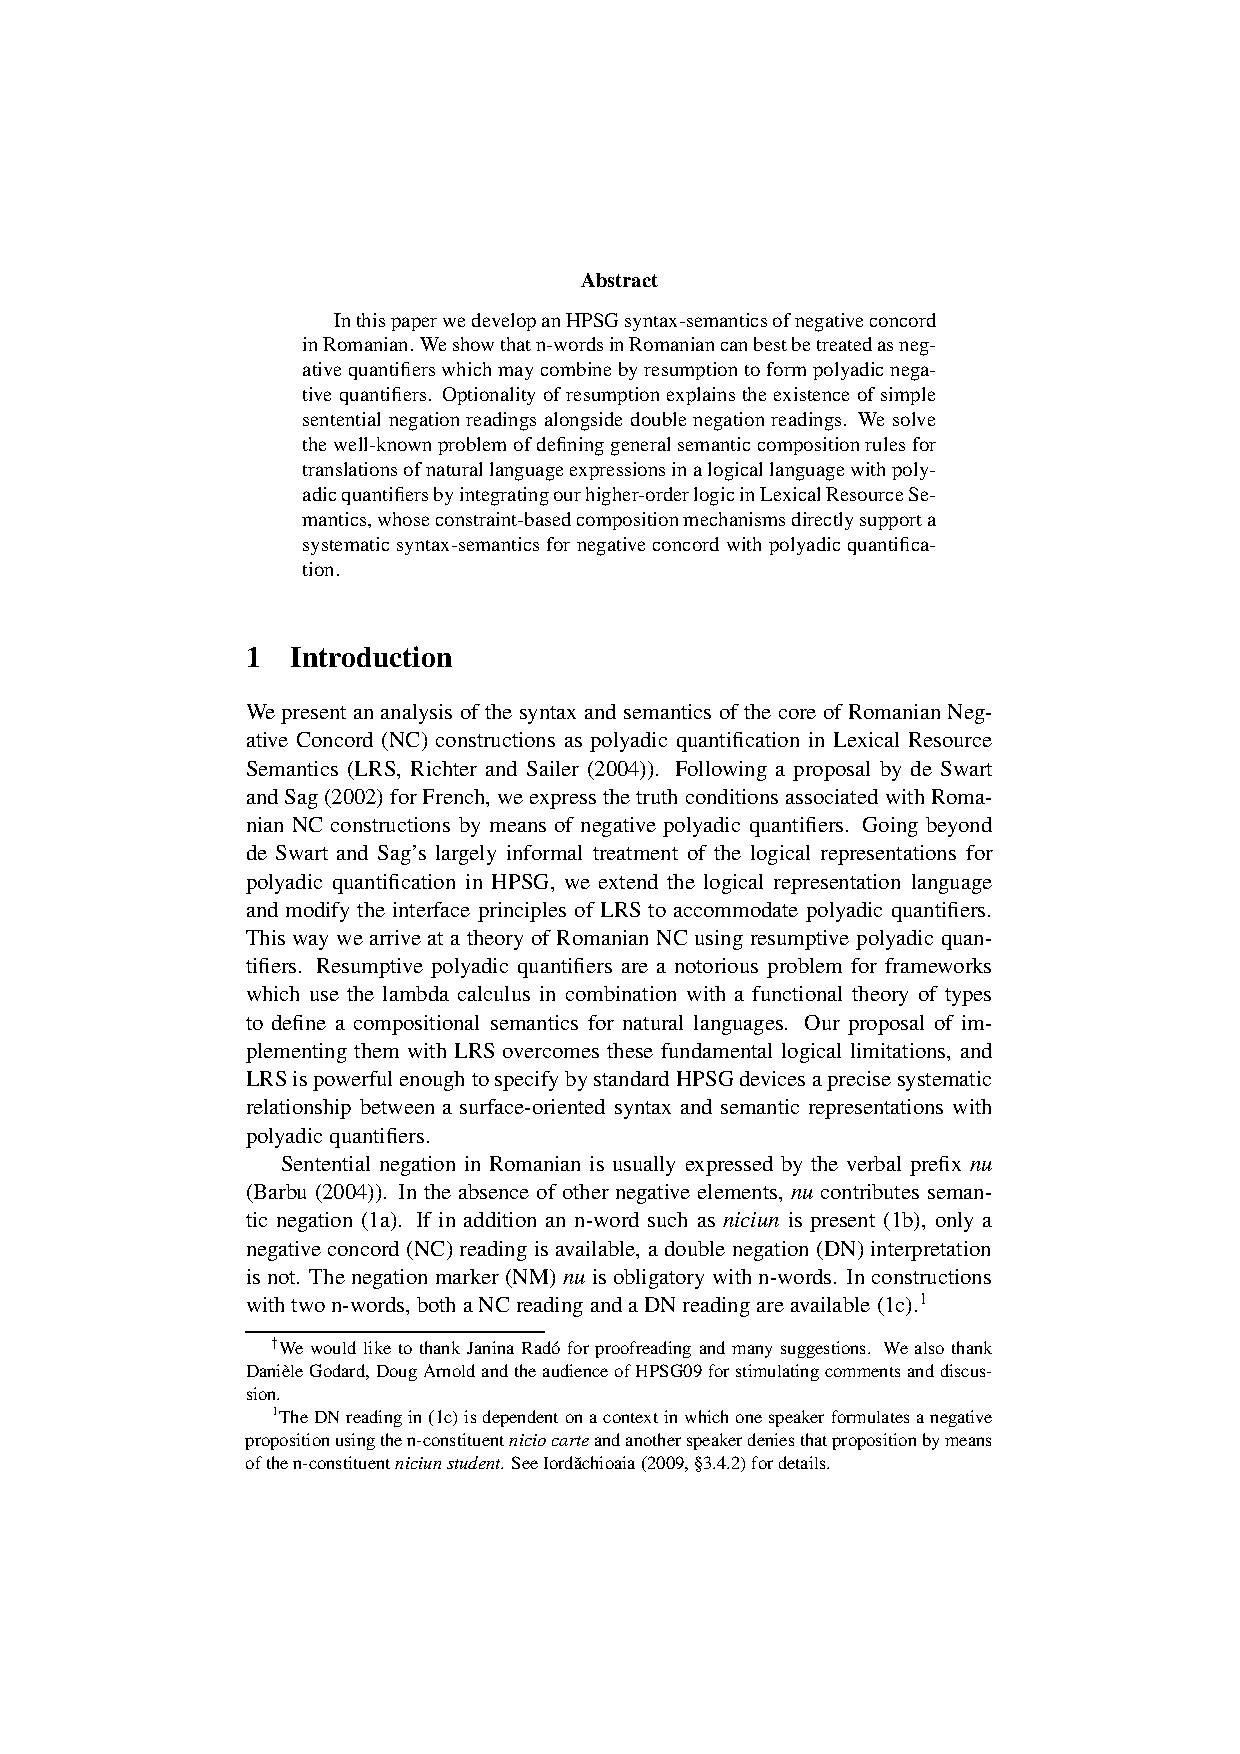
\includepdf[pages=-,pagecommand=\thispagestyle{plain}]{Includes/iordachioaia-richter.pdf}
        \setcounter{page}{171}
        \phantomsection
        \addcontentsline{toc}{section}{Paul Kay, Ivan A. Sag: How Hard a Problem Would This Be to Solve?}
\thispagestyle{empty}

\begin{center}
  {\huge\bfseries How Hard a Problem Would This Be to Solve?\par}

  \bigskip

~\\
\begingroup
\setlength{\leftskip}{0pt plus 1fill}
\setlength{\rightskip}{0pt plus 1fill}
\setlength{\parindent}{0pt}
\setlength{\parfillskip}{0pt}
  \formatauthor{Paul Kay}{\begin{tabular}{@{}c@{}}University of California, Berkeley\end{tabular}}
\formatauthor{Ivan A. Sag}{\begin{tabular}{@{}c@{}}Stanford University\end{tabular}}

\par\endgroup

  \vspace*{8ex}

  Proceedings of the 16th International Conference on\par Head-Driven Phrase Structure Grammar

  \bigskip

  Georg-August-Universit\"{a}t G{\"o}ttingen, Germany

  \medskip

  Stefan Müller (Editor)

  \medskip

  2009

  \medskip

  CSLI Publications

  \medskip

  pages 171--191

  \medskip

  \url{http://csli-publications.stanford.edu/HPSG/2009}
\end{center}
\vfill

\noindent



\vfill
\noindent
% APA Style
Kay, Paul, \& Sag, Ivan A. 2009. How Hard a Problem Would This Be to Solve? In Müller, Stefan (Ed.), \emph{{Proceedings of the 16th International Conference on Head-Driven Phrase Structure Grammar, Georg-August-Universit\"{a}t G{\"o}ttingen, Germany}}, 171--191. Stanford,
CA: CSLI Publications. \hfill\href{http://creativecommons.org/licenses/by/4.0/}{\includegraphics[height=.75em]{Includes/ccby.eps}}

\newpage
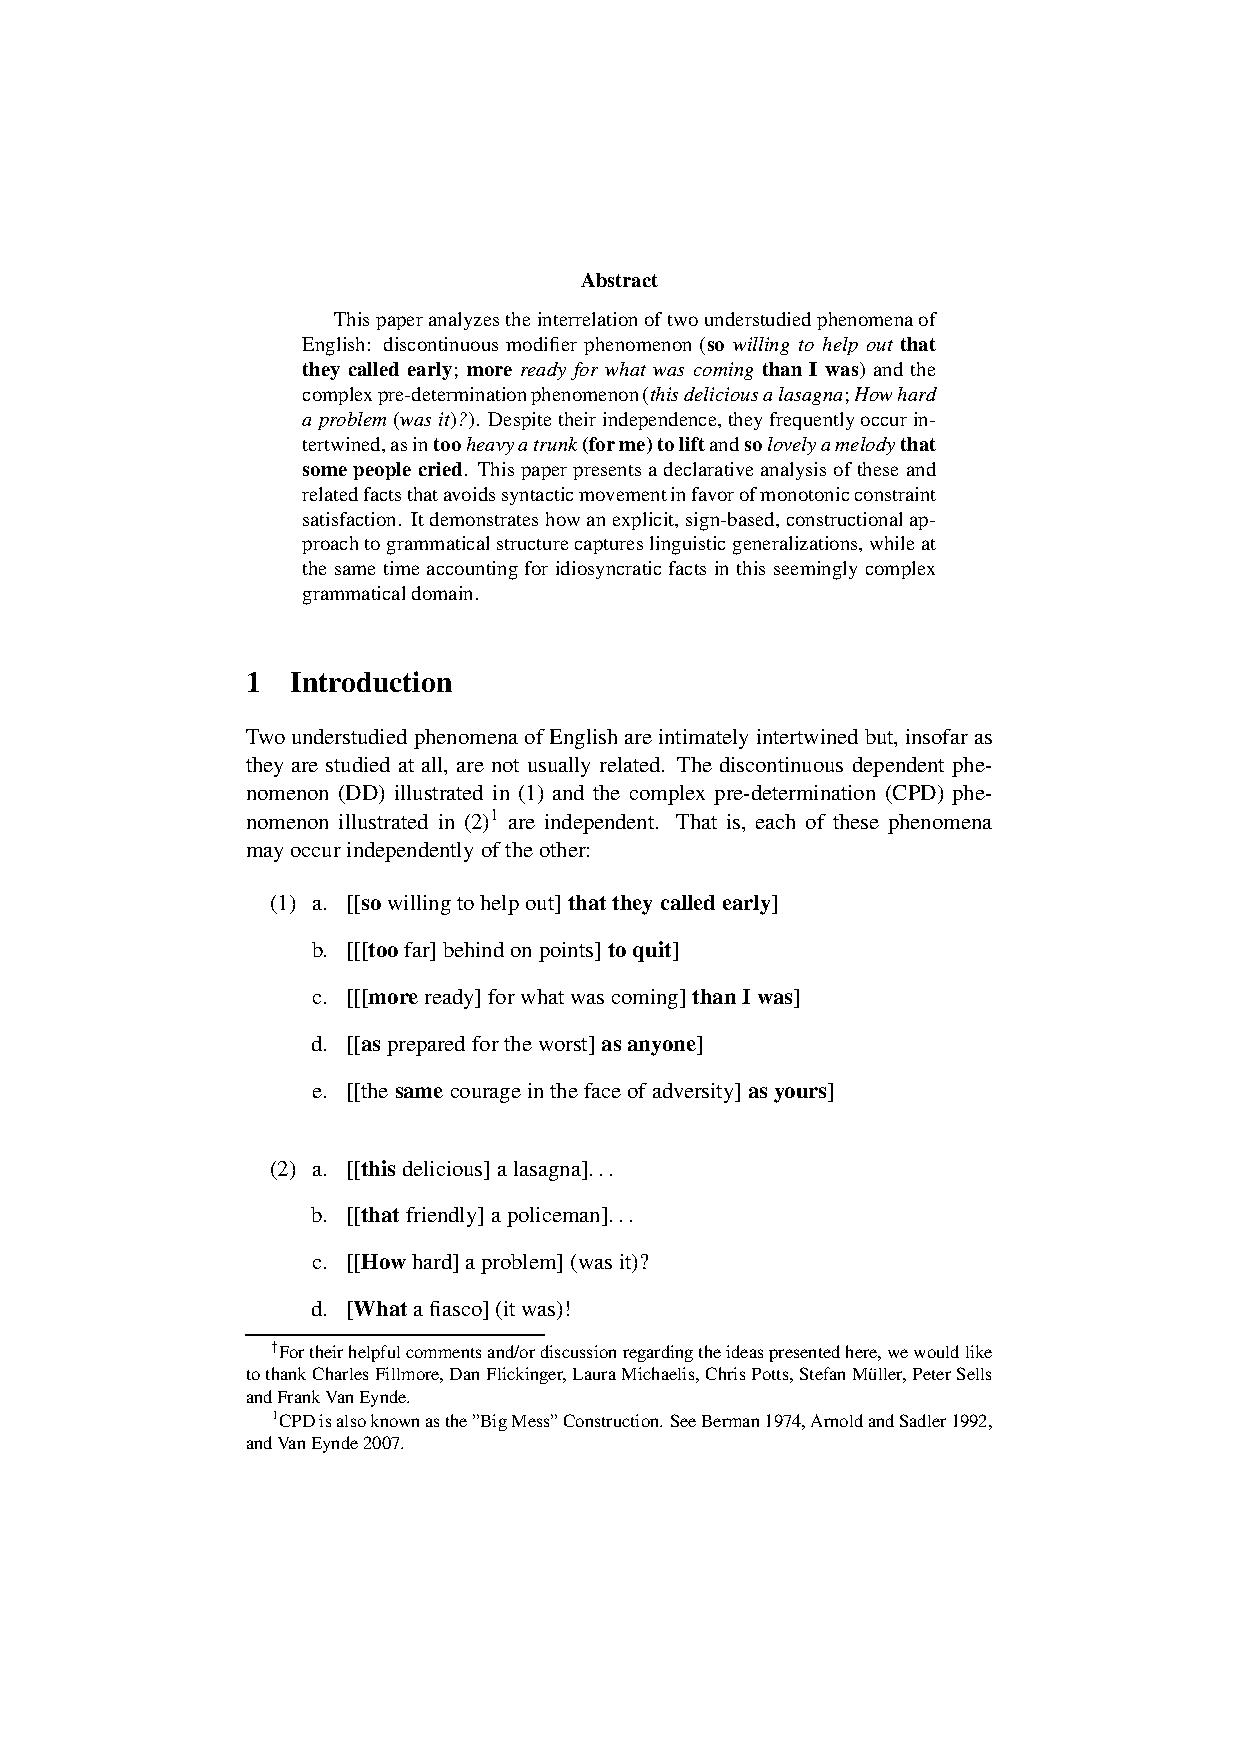
\includepdf[pages=-,pagecommand=\thispagestyle{plain}]{Includes/kay-sag.pdf}
        \setcounter{page}{192}
        \phantomsection
        \addcontentsline{toc}{section}{David Lahm: An Alternative to the HPSG Raising Principle on the Description-Level}
\thispagestyle{empty}

\begin{center}
  {\huge\bfseries An Alternative to the HPSG Raising Principle on the Description-Level\par}

  \bigskip

~\\
\begingroup
\setlength{\leftskip}{0pt plus 1fill}
\setlength{\rightskip}{0pt plus 1fill}
\setlength{\parindent}{0pt}
\setlength{\parfillskip}{0pt}
  \formatauthor{David Lahm}{\begin{tabular}{@{}c@{}}Universität Tübingen\end{tabular}}

\par\endgroup

  \vspace*{8ex}

  Proceedings of the 16th International Conference on\par Head-Driven Phrase Structure Grammar

  \bigskip

  Georg-August-Universit\"{a}t G{\"o}ttingen, Germany

  \medskip

  Stefan Müller (Editor)

  \medskip

  2009

  \medskip

  CSLI Publications

  \medskip

  pages 192--212

  \medskip

  \url{http://csli-publications.stanford.edu/HPSG/2009}
\end{center}
\vfill

\noindent



\vfill
\noindent
% APA Style
Lahm, David. 2009. An Alternative to the HPSG Raising Principle on the Description-Level. In Müller, Stefan (Ed.), \emph{{Proceedings of the 16th International Conference on Head-Driven Phrase Structure Grammar, Georg-August-Universit\"{a}t G{\"o}ttingen, Germany}}, 192--212. Stanford,
CA: CSLI Publications. \hfill\href{http://creativecommons.org/licenses/by/4.0/}{\includegraphics[height=.75em]{Includes/ccby.eps}}

\newpage
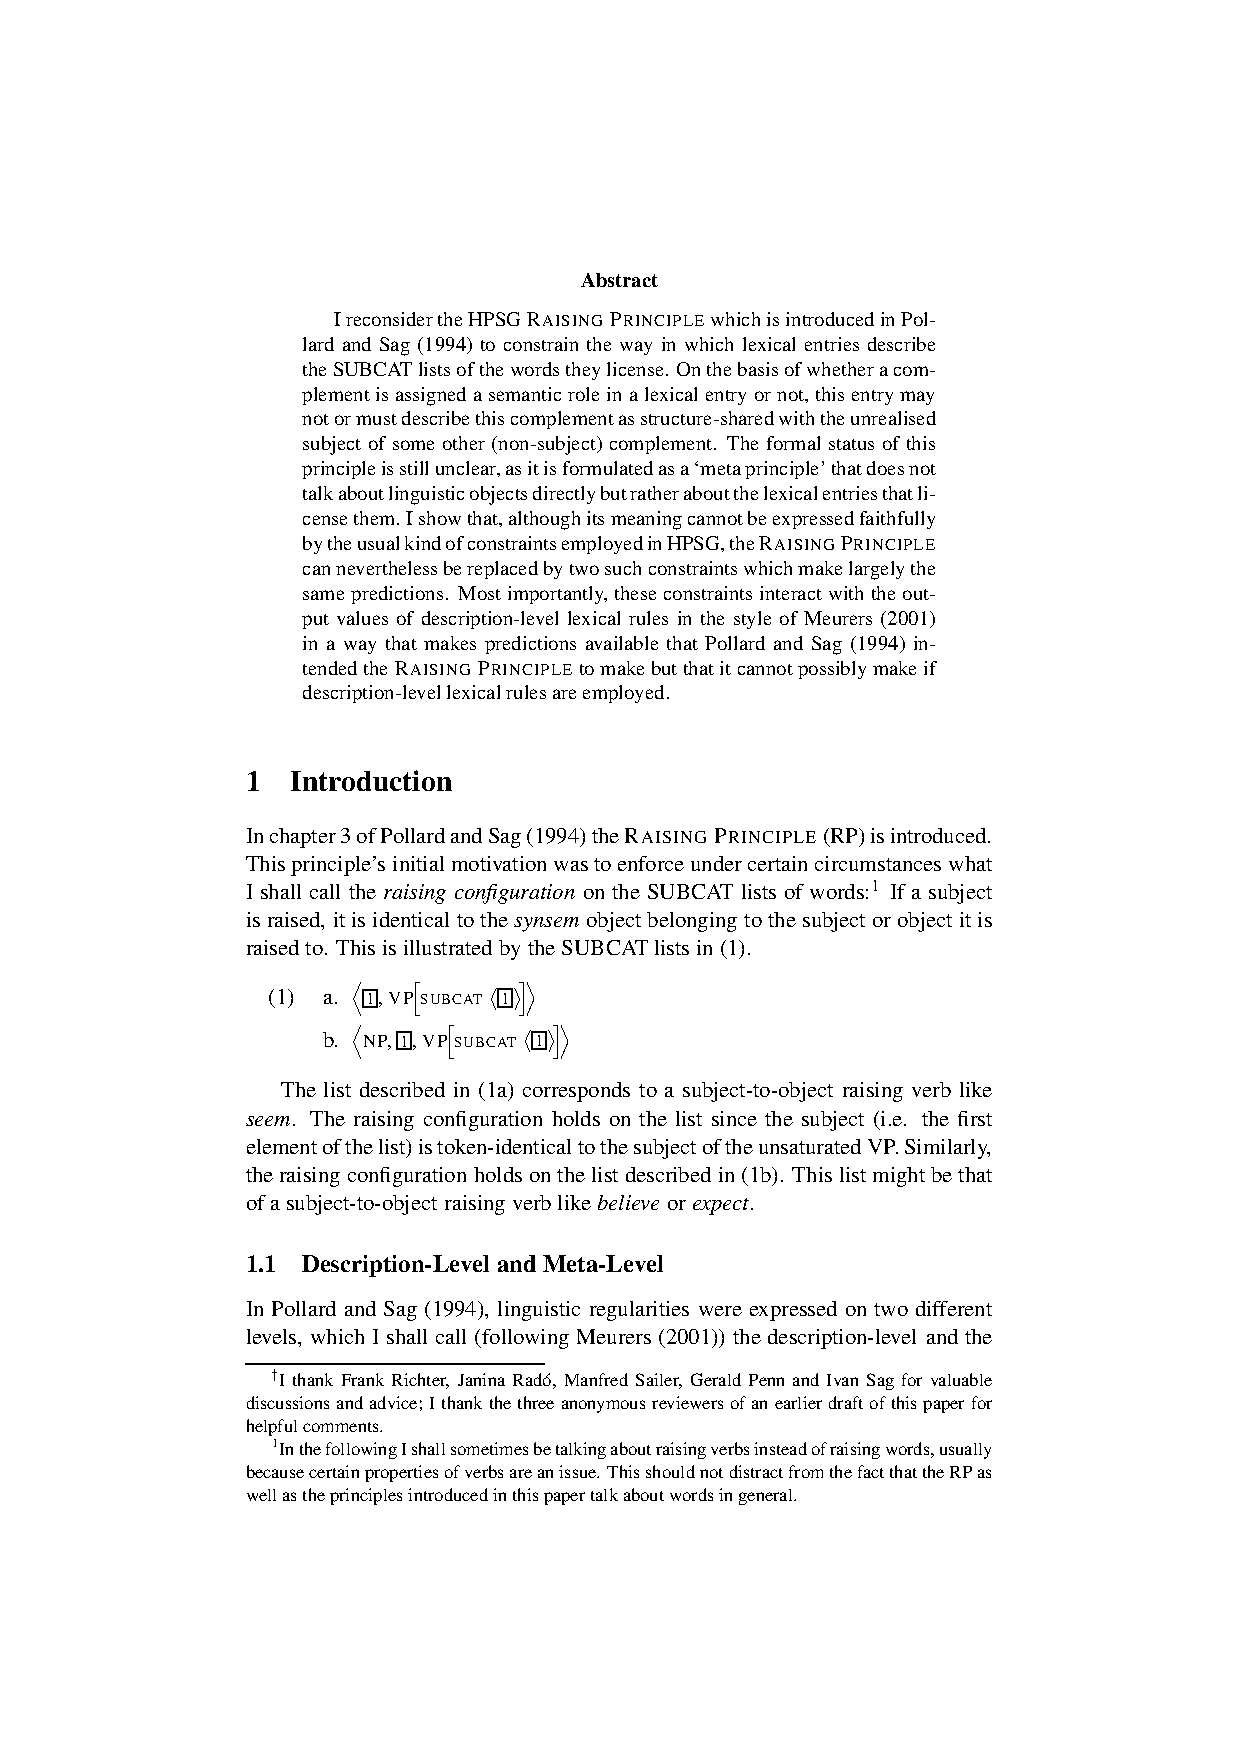
\includepdf[pages=-,pagecommand=\thispagestyle{plain}]{Includes/lahm.pdf}
        \setcounter{page}{213}
        \phantomsection
        \addcontentsline{toc}{section}{Stefan M{\"u}ller: On Predication}
\thispagestyle{empty}

\begin{center}
  {\huge\bfseries On Predication\par}

  \bigskip

~\\
\begingroup
\setlength{\leftskip}{0pt plus 1fill}
\setlength{\rightskip}{0pt plus 1fill}
\setlength{\parindent}{0pt}
\setlength{\parfillskip}{0pt}
  \formatauthor{Stefan Müller}{\begin{tabular}{@{}c@{}}Freie Universität Berlin\end{tabular}}

\par\endgroup

  \vspace*{8ex}

  Proceedings of the 16th International Conference on\par Head-Driven Phrase Structure Grammar

  \bigskip

  Georg-August-Universit\"{a}t G{\"o}ttingen, Germany

  \medskip

  Stefan Müller (Editor)

  \medskip

  2009

  \medskip

  CSLI Publications

  \medskip

  pages 213--233

  \medskip

  \url{http://csli-publications.stanford.edu/HPSG/2009}
\end{center}
\vfill

\noindent



\vfill
\noindent
% APA Style
Müller, Stefan. 2009. On Predication. In Müller, Stefan (Ed.), \emph{{Proceedings of the 16th International Conference on Head-Driven Phrase Structure Grammar, Georg-August-Universit\"{a}t G{\"o}ttingen, Germany}}, 213--233. Stanford,
CA: CSLI Publications. \hfill\href{http://creativecommons.org/licenses/by/4.0/}{\includegraphics[height=.75em]{Includes/ccby.eps}}

\newpage
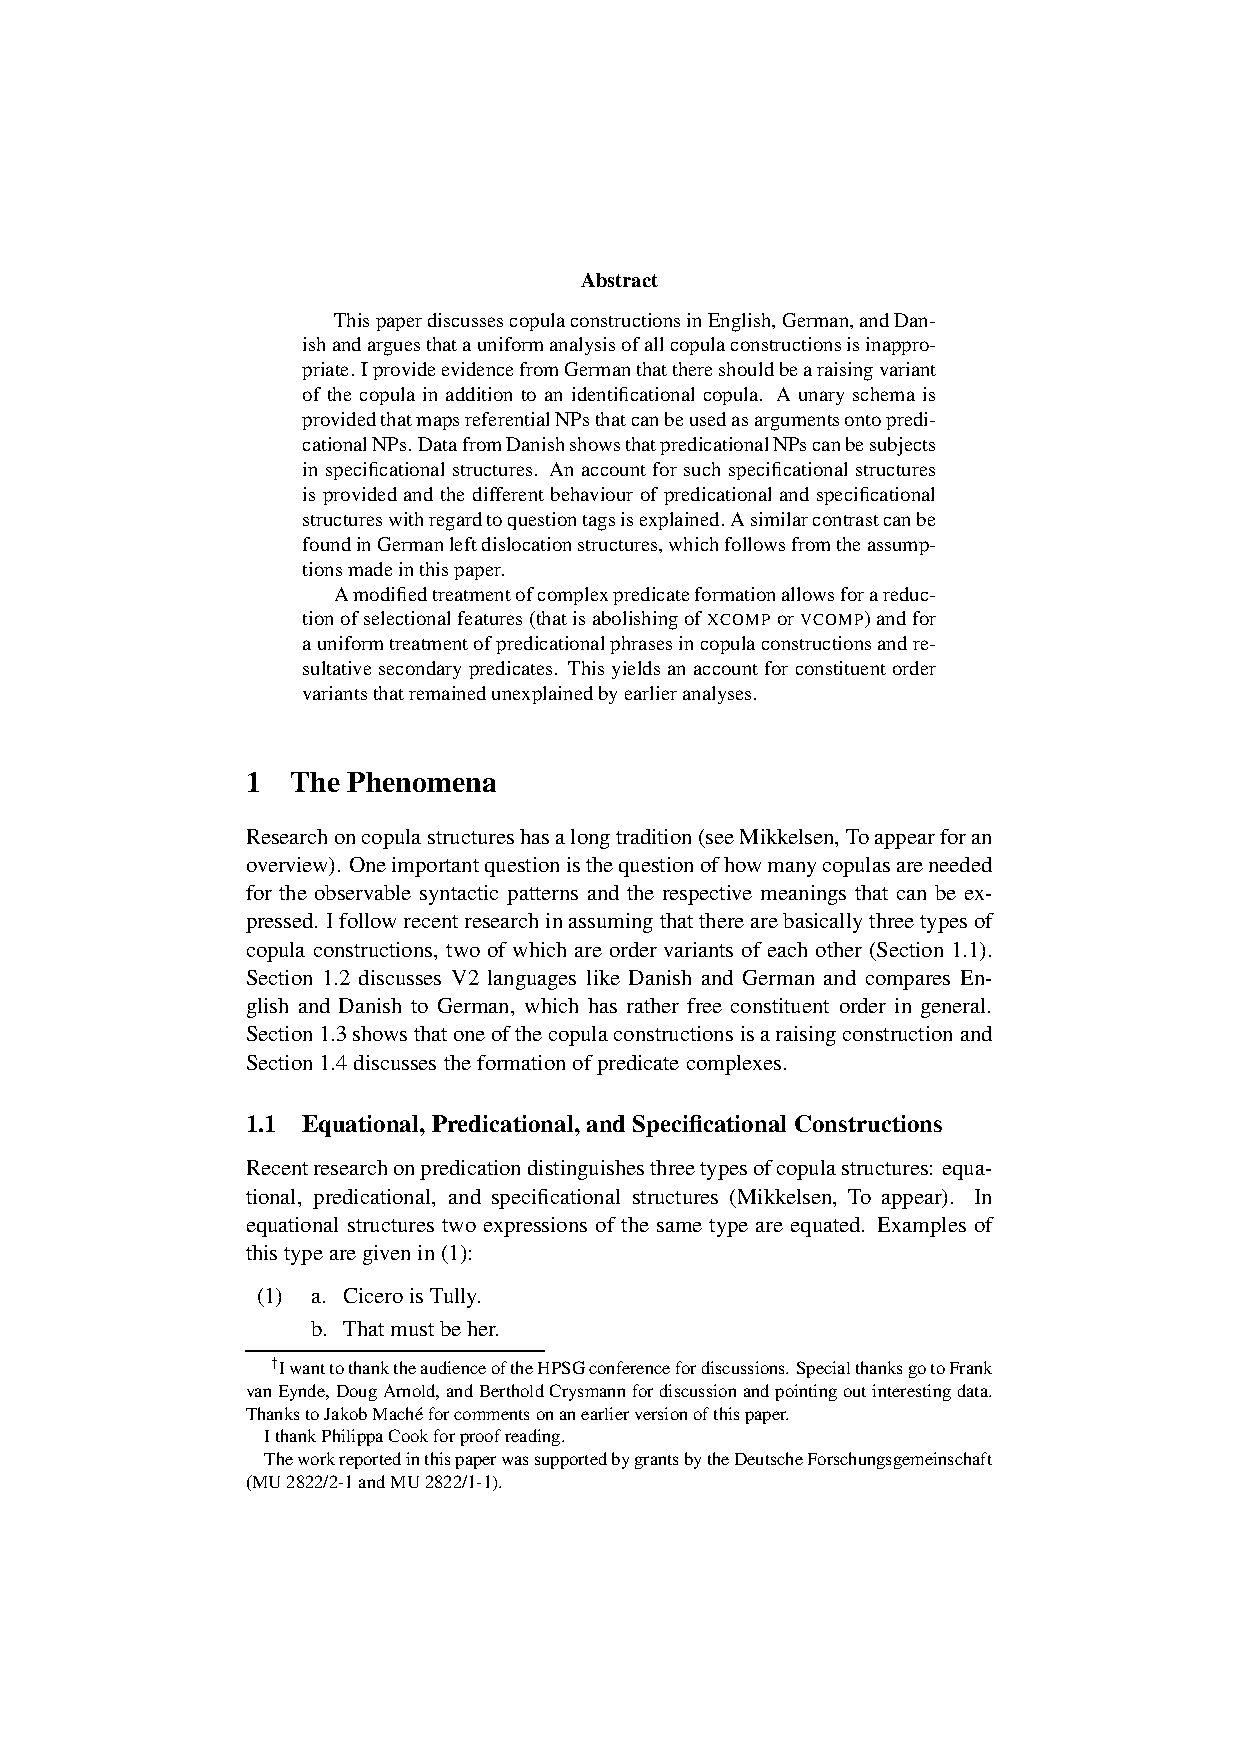
\includepdf[pages=-,pagecommand=\thispagestyle{plain}]{Includes/mueller.pdf}
        \setcounter{page}{234}
        \phantomsection
        \addcontentsline{toc}{section}{Stefan M{\"u}ller, Janna Lipenkova: Serial Verb Constructions in Chinese:\\ A HPSG Account}
\thispagestyle{empty}

\begin{center}
  {\huge\bfseries Serial Verb Constructions in Chinese:\par A HPSG Account\par}

  \bigskip

~\\
\begingroup
\setlength{\leftskip}{0pt plus 1fill}
\setlength{\rightskip}{0pt plus 1fill}
\setlength{\parindent}{0pt}
\setlength{\parfillskip}{0pt}
  \formatauthor{Stefan Müller}{\begin{tabular}{@{}c@{}}Freie Universität Berlin\end{tabular}}
\formatauthor{Janna Lipenkova}{\begin{tabular}{@{}c@{}}Freie Universität Berlin\end{tabular}}

\par\endgroup

  \vspace*{8ex}

  Proceedings of the 16th International Conference on\par Head-Driven Phrase Structure Grammar

  \bigskip

  Georg-August-Universit\"{a}t G{\"o}ttingen, Germany

  \medskip

  Stefan Müller (Editor)

  \medskip

  2009

  \medskip

  CSLI Publications

  \medskip

  pages 234--254

  \medskip

  \url{http://csli-publications.stanford.edu/HPSG/2009}
\end{center}
\vfill

\noindent



\vfill
\noindent
% APA Style
Müller, Stefan, \& Lipenkova, Janna. 2009. Serial Verb Constructions in Chinese:  A HPSG Account. In Müller, Stefan (Ed.), \emph{{Proceedings of the 16th International Conference on Head-Driven Phrase Structure Grammar, Georg-August-Universit\"{a}t G{\"o}ttingen, Germany}}, 234--254. Stanford,
CA: CSLI Publications. \hfill\href{http://creativecommons.org/licenses/by/4.0/}{\includegraphics[height=.75em]{Includes/ccby.eps}}

\newpage
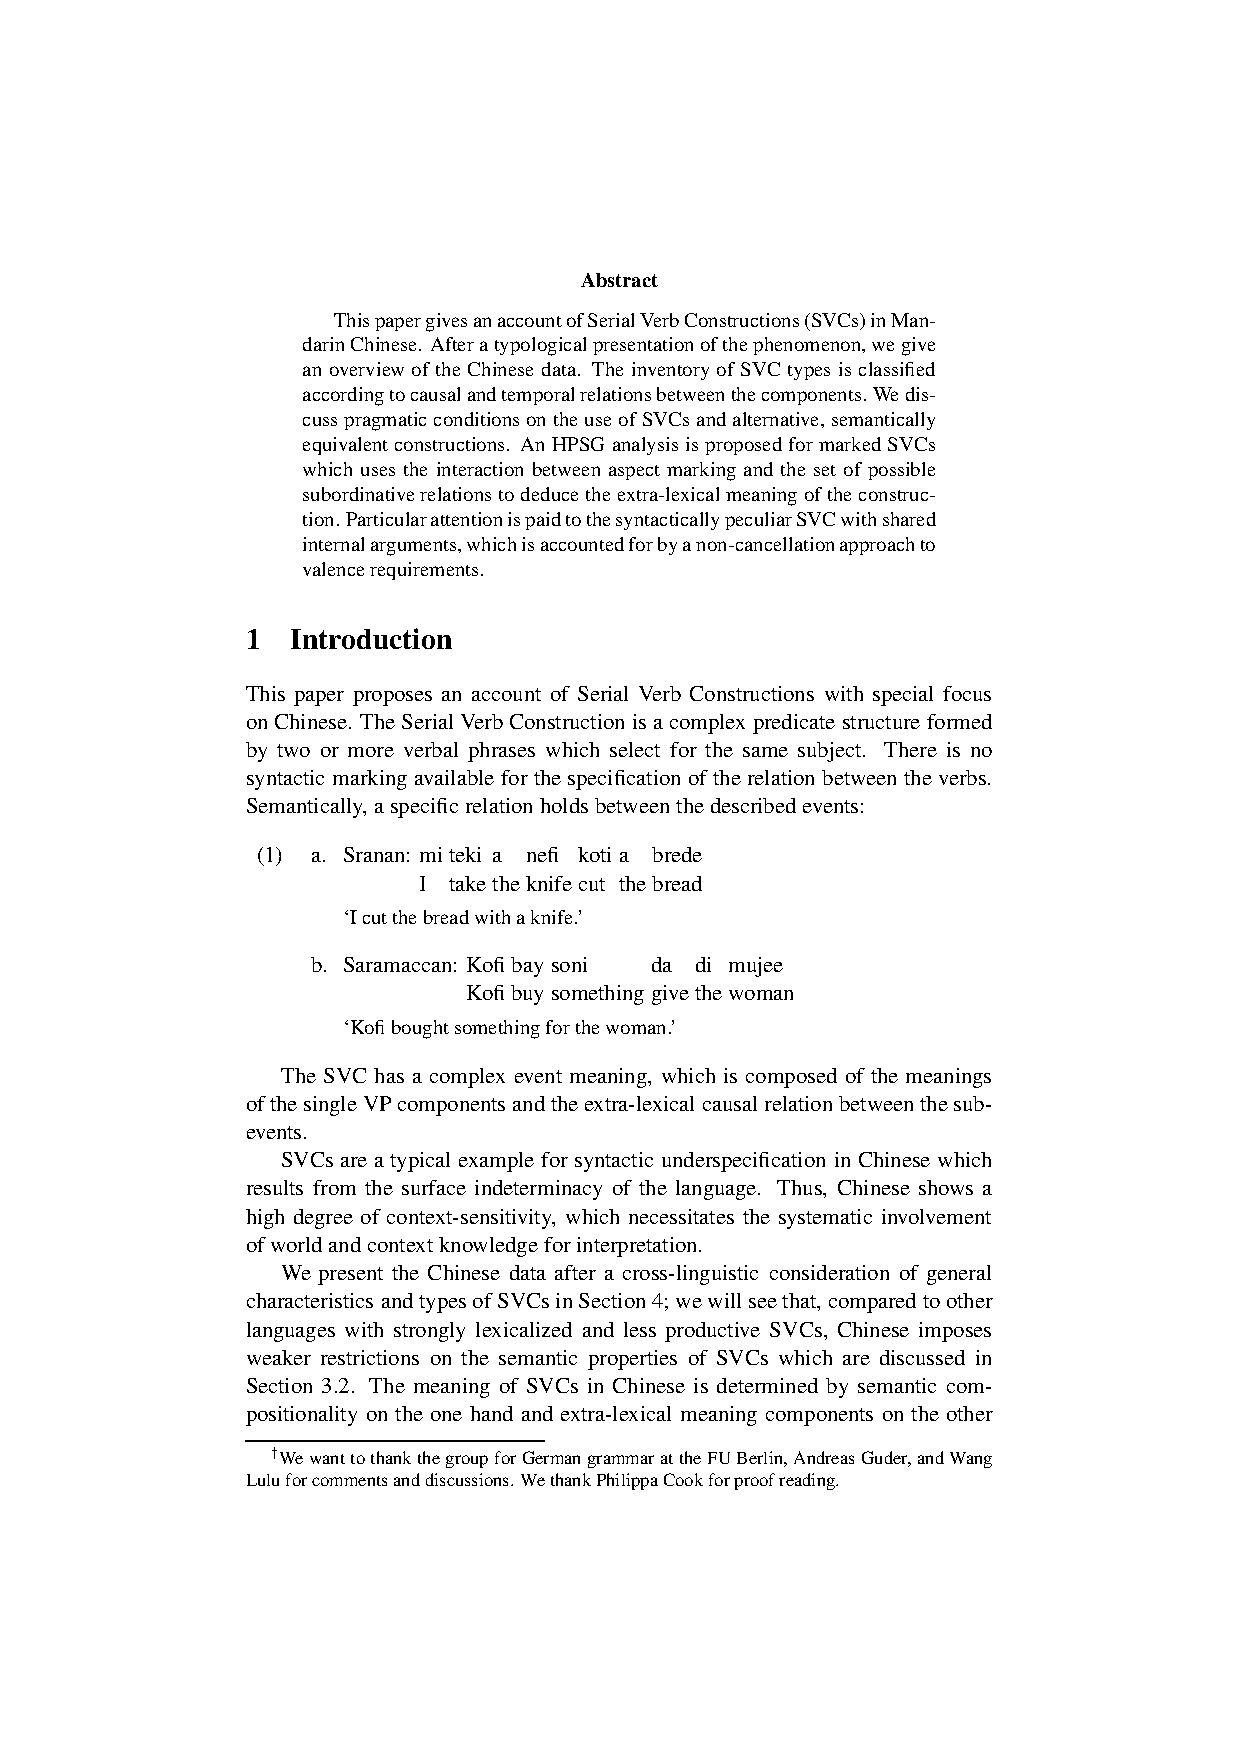
\includepdf[pages=-,pagecommand=\thispagestyle{plain}]{Includes/mueller-lipenkova.pdf}
        \setcounter{page}{255}
        \phantomsection
        \addcontentsline{toc}{section}{Bjarne {\O}rsnes: Preposed Negation in Danish}
\thispagestyle{empty}

\begin{center}
  {\huge\bfseries Preposed Negation in Danish\par}

  \bigskip

~\\
\begingroup
\setlength{\leftskip}{0pt plus 1fill}
\setlength{\rightskip}{0pt plus 1fill}
\setlength{\parindent}{0pt}
\setlength{\parfillskip}{0pt}
  \formatauthor{Bjarne Ørsnes}{\begin{tabular}{@{}c@{}}Freie Universität Berlin\end{tabular}}

\par\endgroup

  \vspace*{8ex}

  Proceedings of the 16th International Conference on\par Head-Driven Phrase Structure Grammar

  \bigskip

  Georg-August-Universit\"{a}t G{\"o}ttingen, Germany

  \medskip

  Stefan Müller (Editor)

  \medskip

  2009

  \medskip

  CSLI Publications

  \medskip

  pages 255--275

  \medskip

  \url{http://csli-publications.stanford.edu/HPSG/2009}
\end{center}
\vfill

\noindent



\vfill
\noindent
% APA Style
Ørsnes, Bjarne. 2009. Preposed Negation in Danish. In Müller, Stefan (Ed.), \emph{{Proceedings of the 16th International Conference on Head-Driven Phrase Structure Grammar, Georg-August-Universit\"{a}t G{\"o}ttingen, Germany}}, 255--275. Stanford,
CA: CSLI Publications. \hfill\href{http://creativecommons.org/licenses/by/4.0/}{\includegraphics[height=.75em]{Includes/ccby.eps}}

\newpage
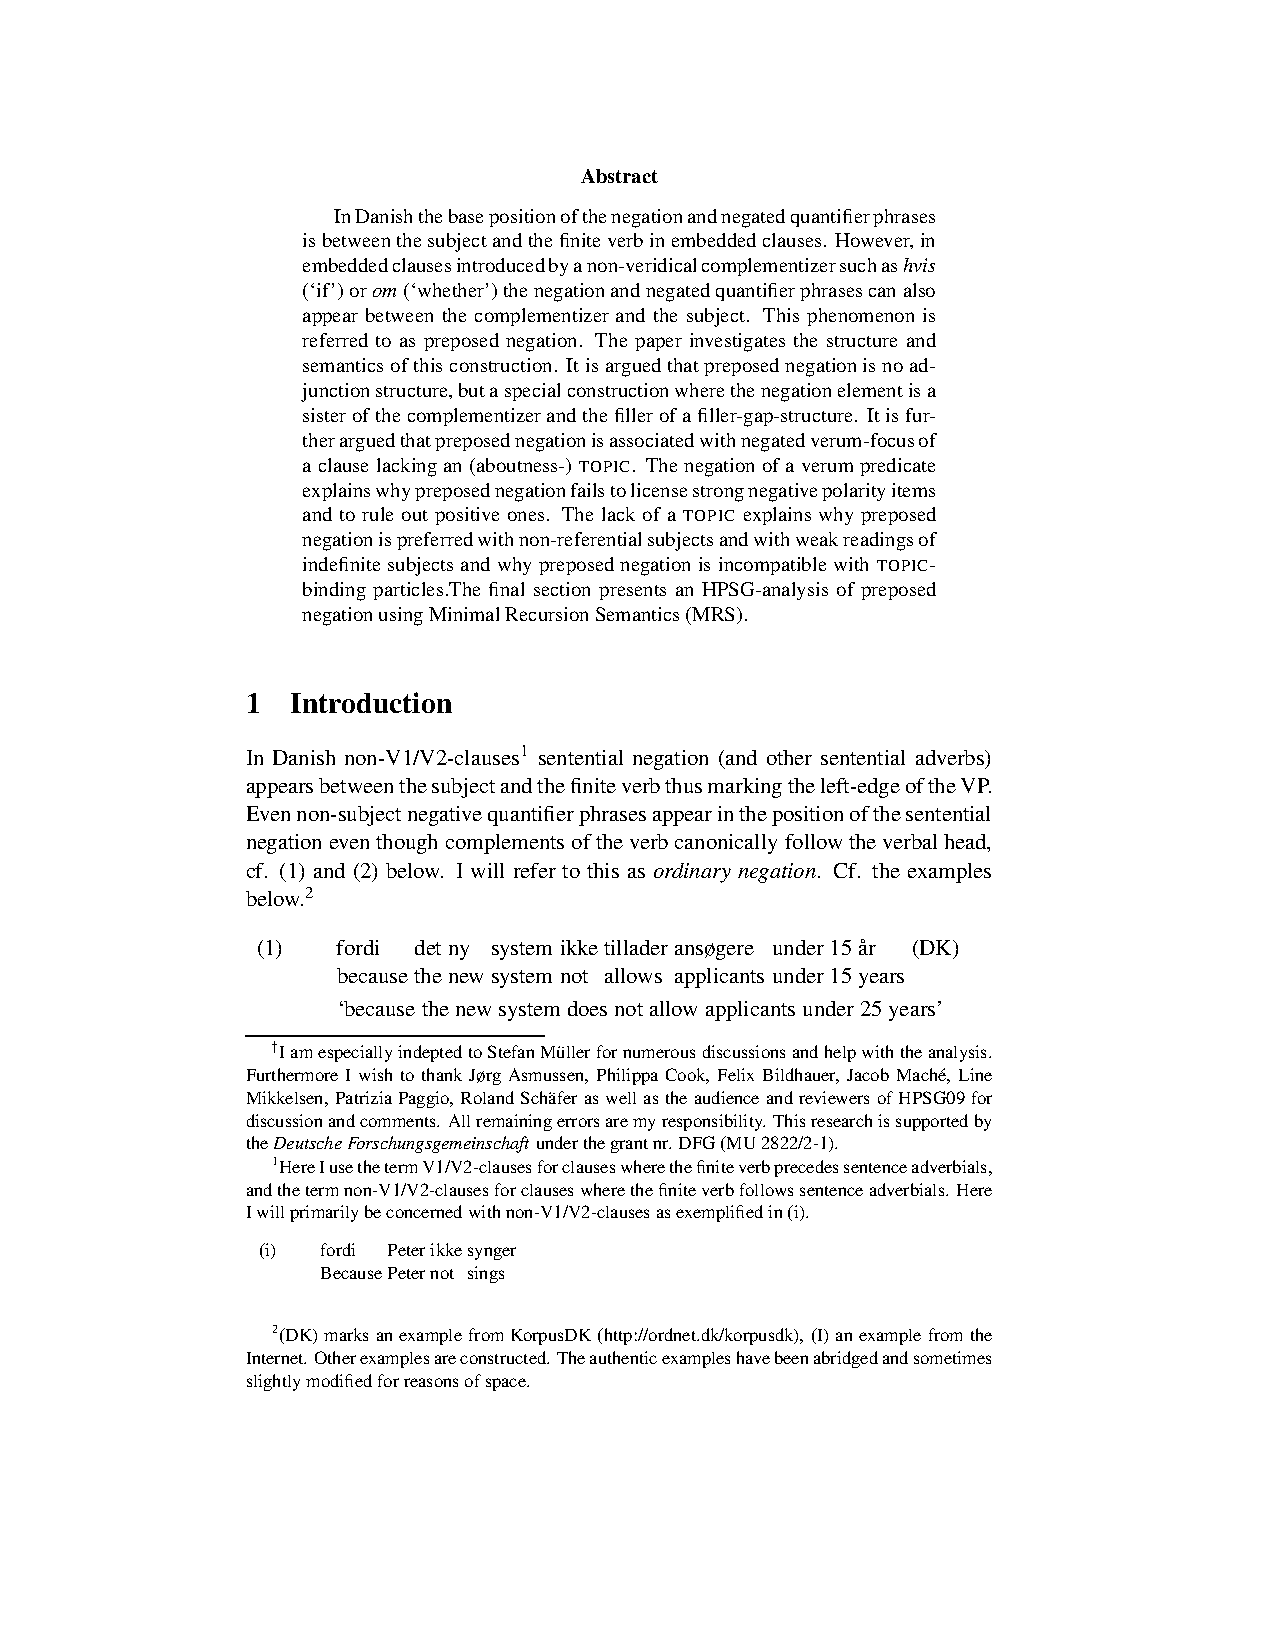
\includepdf[pages=-,pagecommand=\thispagestyle{plain}]{Includes/oersnes.pdf}
        \setcounter{page}{276}
        \phantomsection
        \addcontentsline{toc}{section}{Shakthi Poornima, Jean-Pierre Koenig: Hindi Aspectual Complex Predicates}
\thispagestyle{empty}

\begin{center}
  {\huge\bfseries Hindi Aspectual Complex Predicates\par}

  \bigskip

~\\
\begingroup
\setlength{\leftskip}{0pt plus 1fill}
\setlength{\rightskip}{0pt plus 1fill}
\setlength{\parindent}{0pt}
\setlength{\parfillskip}{0pt}
  \formatauthor{Shakthi Poornima}{\begin{tabular}{@{}c@{}}State University of New York at Buffalo\end{tabular}}
\formatauthor{Jean-Pierre Koenig}{\begin{tabular}{@{}c@{}}State University of New York at Buffalo\end{tabular}}

\par\endgroup

  \vspace*{8ex}

  Proceedings of the 16th International Conference on\par Head-Driven Phrase Structure Grammar

  \bigskip

  Georg-August-Universit\"{a}t G{\"o}ttingen, Germany

  \medskip

  Stefan Müller (Editor)

  \medskip

  2009

  \medskip

  CSLI Publications

  \medskip

  pages 276--296

  \medskip

  \url{http://csli-publications.stanford.edu/HPSG/2009}
\end{center}
\vfill

\noindent



\vfill
\noindent
% APA Style
Poornima, Shakthi, \& Koenig, Jean-Pierre. 2009. Hindi Aspectual Complex Predicates. In Müller, Stefan (Ed.), \emph{{Proceedings of the 16th International Conference on Head-Driven Phrase Structure Grammar, Georg-August-Universit\"{a}t G{\"o}ttingen, Germany}}, 276--296. Stanford,
CA: CSLI Publications. \hfill\href{http://creativecommons.org/licenses/by/4.0/}{\includegraphics[height=.75em]{Includes/ccby.eps}}

\newpage
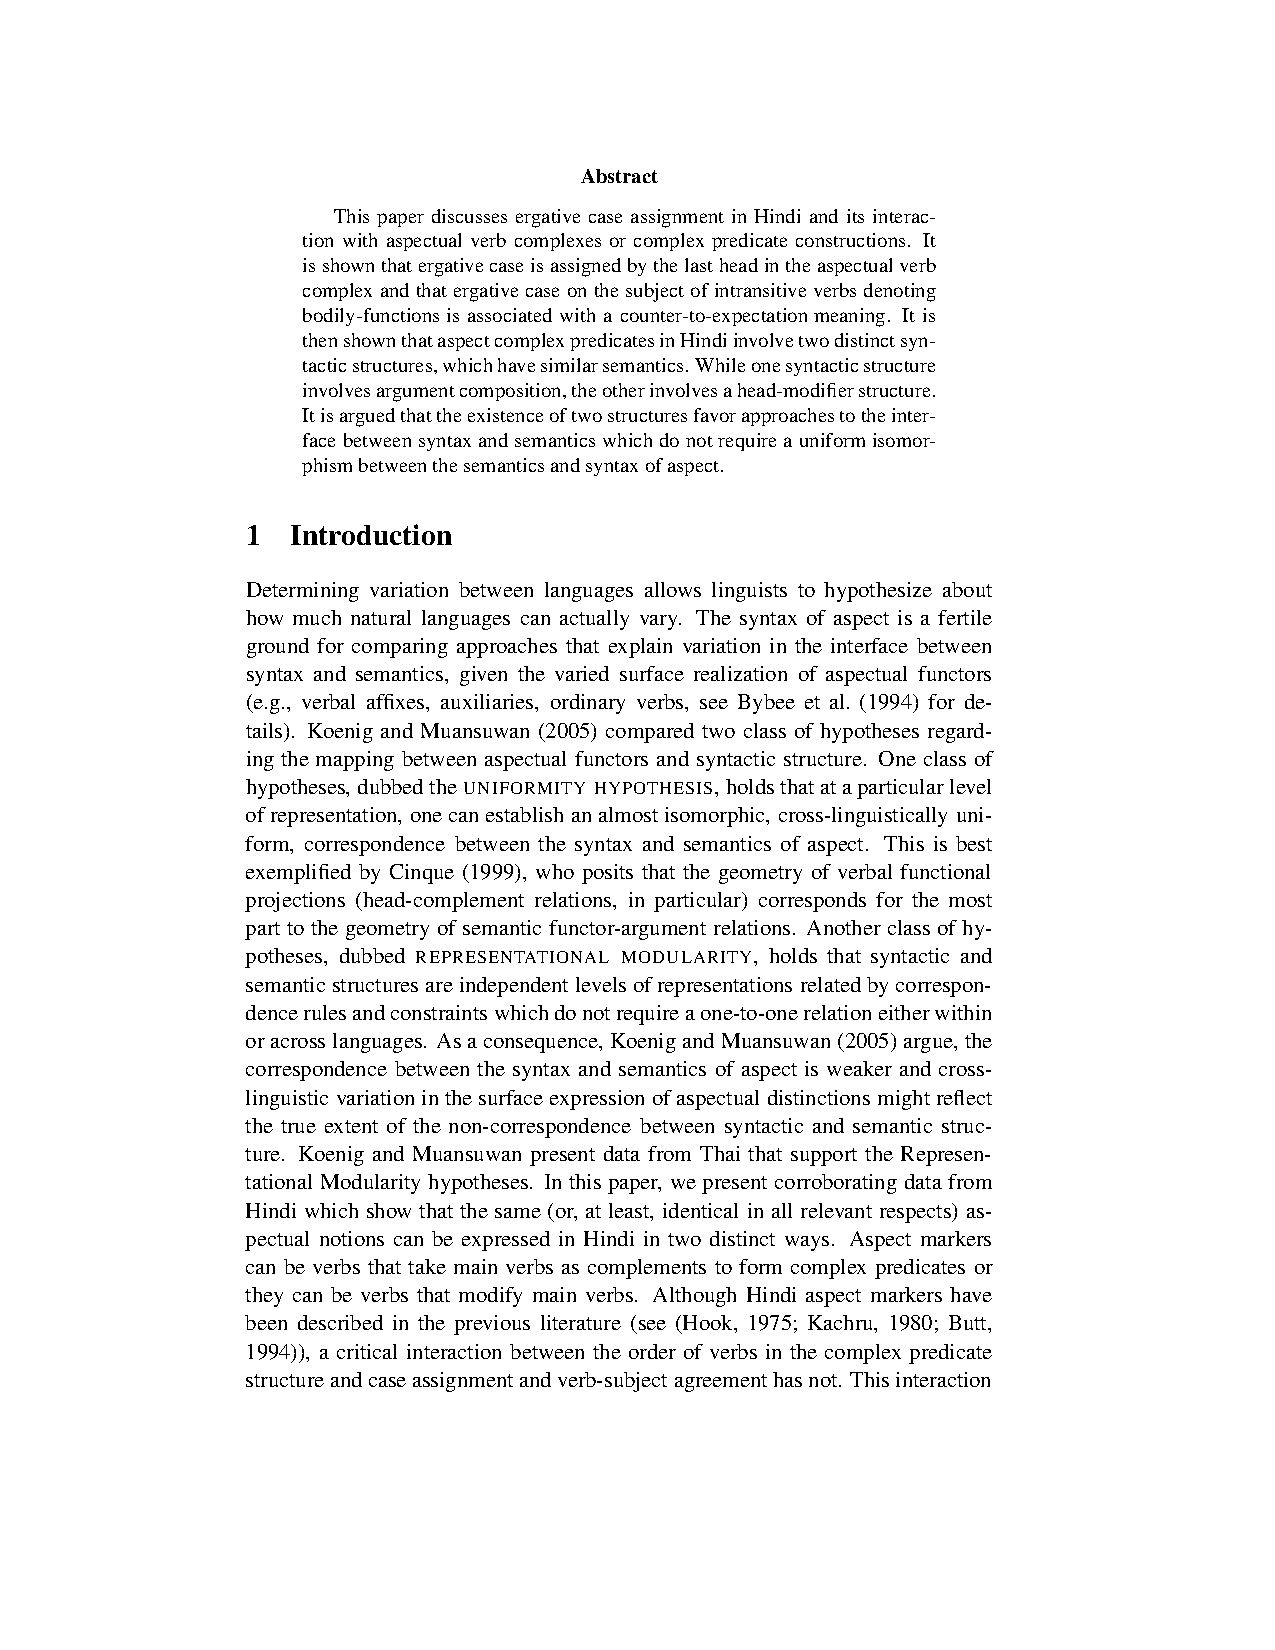
\includepdf[pages=-,pagecommand=\thispagestyle{plain}]{Includes/poornima-koenig.pdf}
        \setcounter{page}{297}
        \phantomsection
        \addcontentsline{toc}{section}{Frank Richter, Manfred Sailer: Phraseological Clauses in Constructional HPSG}
\thispagestyle{empty}

\begin{center}
  {\huge\bfseries Phraseological Clauses in Constructional HPSG\par}

  \bigskip

~\\
\begingroup
\setlength{\leftskip}{0pt plus 1fill}
\setlength{\rightskip}{0pt plus 1fill}
\setlength{\parindent}{0pt}
\setlength{\parfillskip}{0pt}
  \formatauthor{Frank Richter}{\begin{tabular}{@{}c@{}}University of Tübingen\end{tabular}}
\formatauthor{Manfred Sailer}{\begin{tabular}{@{}c@{}}University of Göttingen\end{tabular}}

\par\endgroup

  \vspace*{8ex}

  Proceedings of the 16th International Conference on\par Head-Driven Phrase Structure Grammar

  \bigskip

  Georg-August-Universit\"{a}t G{\"o}ttingen, Germany

  \medskip

  Stefan Müller (Editor)

  \medskip

  2009

  \medskip

  CSLI Publications

  \medskip

  pages 297--317

  \medskip

  \url{http://csli-publications.stanford.edu/HPSG/2009}
\end{center}
\vfill

\noindent



\vfill
\noindent
% APA Style
Richter, Frank, \& Sailer, Manfred. 2009. Phraseological Clauses in Constructional HPSG. In Müller, Stefan (Ed.), \emph{{Proceedings of the 16th International Conference on Head-Driven Phrase Structure Grammar, Georg-August-Universit\"{a}t G{\"o}ttingen, Germany}}, 297--317. Stanford,
CA: CSLI Publications. \hfill\href{http://creativecommons.org/licenses/by/4.0/}{\includegraphics[height=.75em]{Includes/ccby.eps}}

\newpage
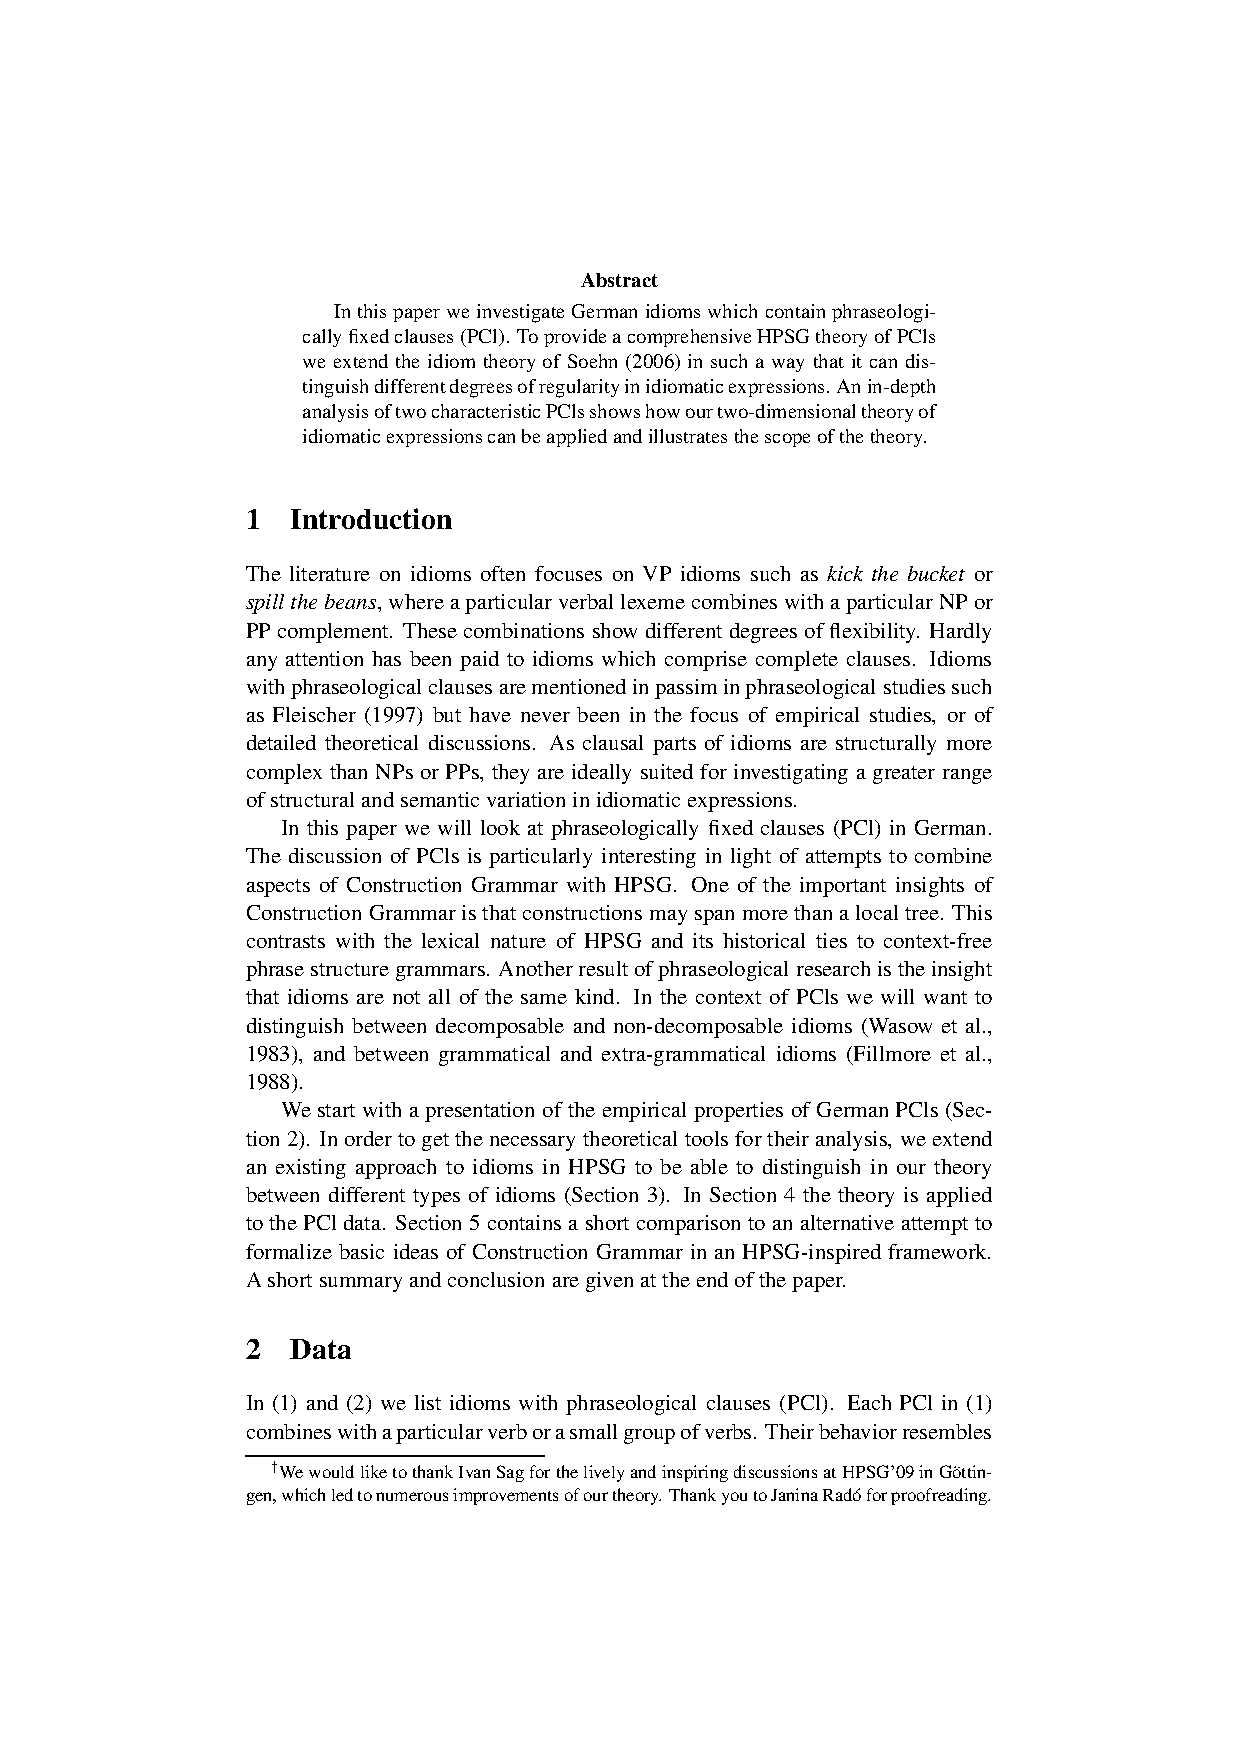
\includepdf[pages=-,pagecommand=\thispagestyle{plain}]{Includes/richter-sailer.pdf}
        \setcounter{page}{318}
        \phantomsection
        \addcontentsline{toc}{section}{Filip Skwarski: Accounting for Underlying Forms in HPSG Phonology}
\thispagestyle{empty}

\begin{center}
  {\huge\bfseries Accounting for Underlying Forms in HPSG Phonology\par}

  \bigskip

~\\
\begingroup
\setlength{\leftskip}{0pt plus 1fill}
\setlength{\rightskip}{0pt plus 1fill}
\setlength{\parindent}{0pt}
\setlength{\parfillskip}{0pt}
  \formatauthor{Filip Skwarski}{\begin{tabular}{@{}c@{}}University of Warsaw\end{tabular}}

\par\endgroup

  \vspace*{8ex}

  Proceedings of the 16th International Conference on\par Head-Driven Phrase Structure Grammar

  \bigskip

  Georg-August-Universit\"{a}t G{\"o}ttingen, Germany

  \medskip

  Stefan Müller (Editor)

  \medskip

  2009

  \medskip

  CSLI Publications

  \medskip

  pages 318--337

  \medskip

  \url{http://csli-publications.stanford.edu/HPSG/2009}
\end{center}
\vfill

\noindent



\vfill
\noindent
% APA Style
Skwarski, Filip. 2009. Accounting for Underlying Forms in HPSG Phonology. In Müller, Stefan (Ed.), \emph{{Proceedings of the 16th International Conference on Head-Driven Phrase Structure Grammar, Georg-August-Universit\"{a}t G{\"o}ttingen, Germany}}, 318--337. Stanford,
CA: CSLI Publications. \hfill\href{http://creativecommons.org/licenses/by/4.0/}{\includegraphics[height=.75em]{Includes/ccby.eps}}

\newpage
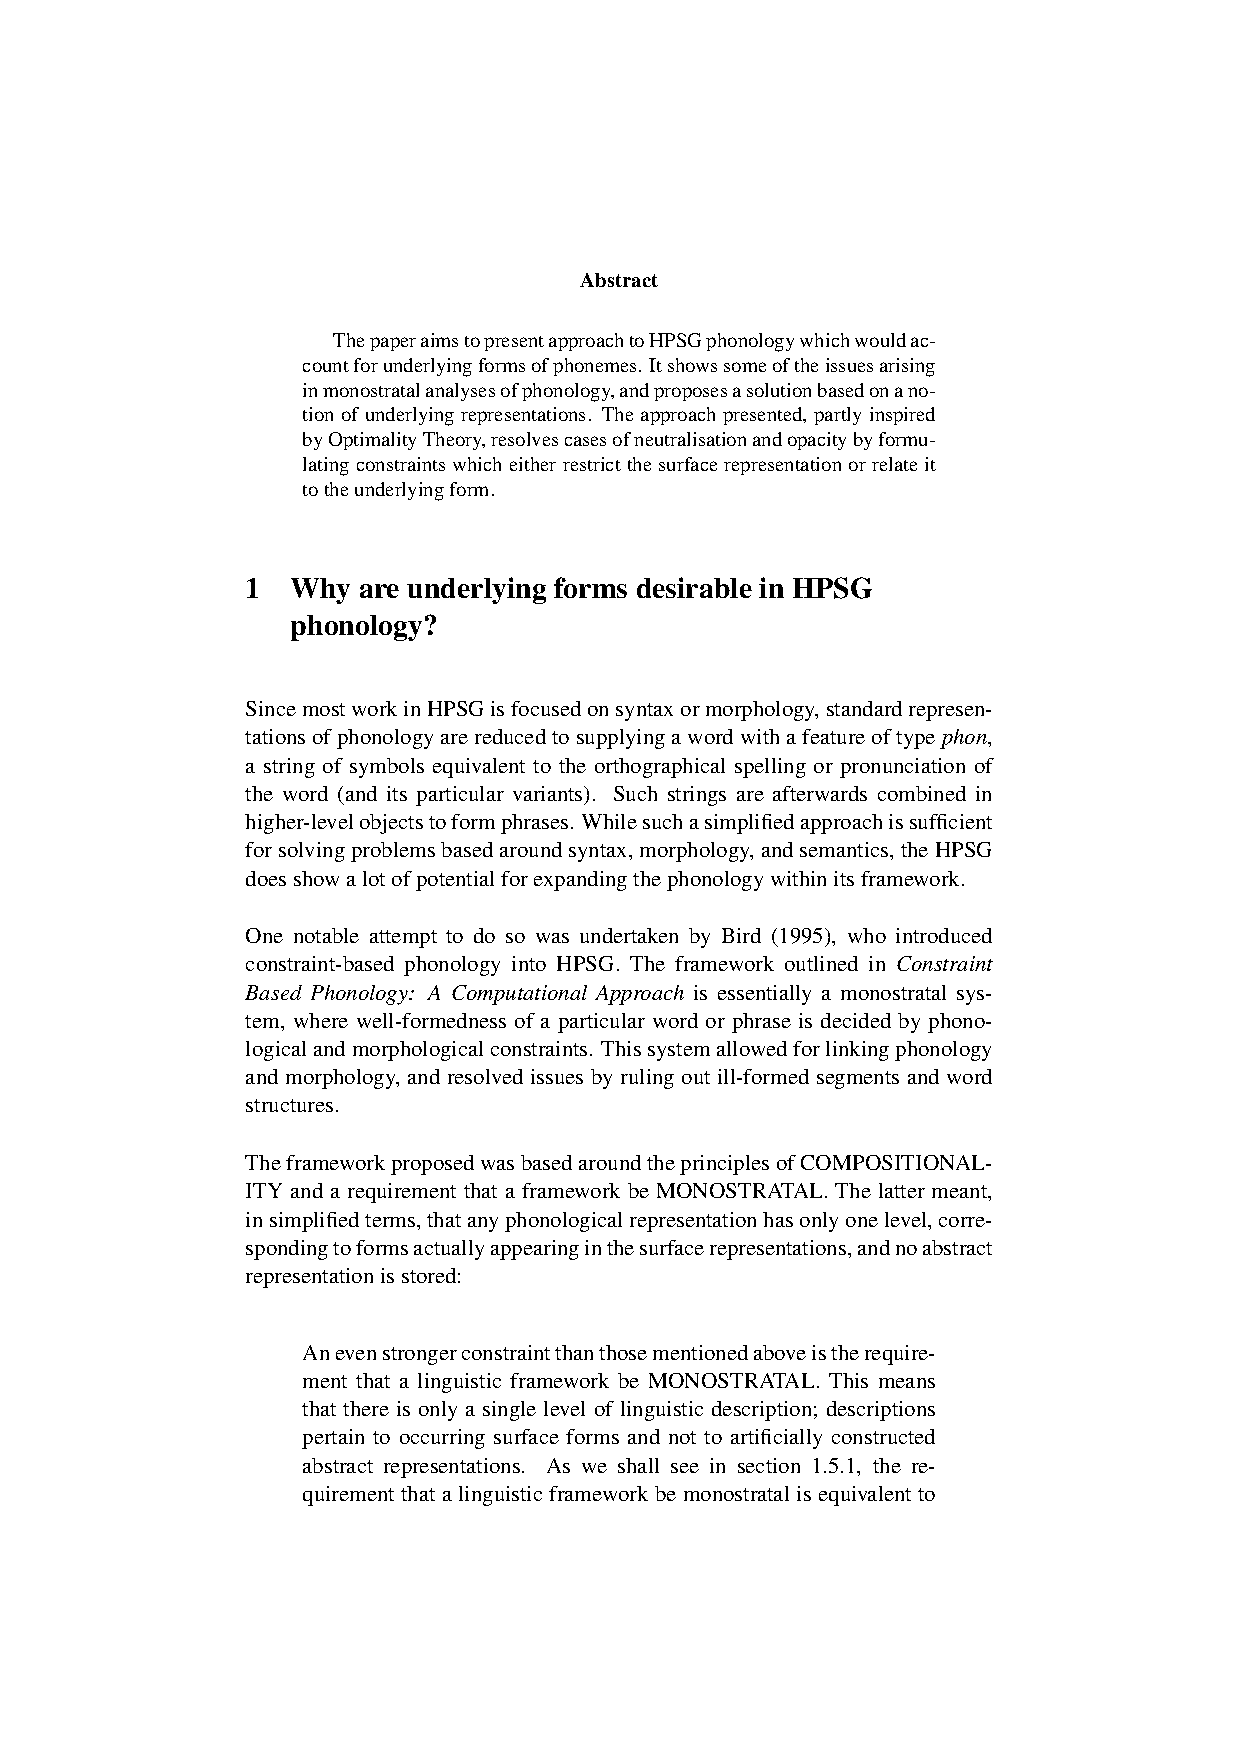
\includepdf[pages=-,pagecommand=\thispagestyle{plain}]{Includes/skwarski.pdf}
        \setcounter{page}{338}
        \phantomsection
        \addcontentsline{toc}{section}{Jesse Tseng: Phonological change and grammaticalization in HPSG: The case of French final consonants}
\thispagestyle{empty}

\begin{center}
  {\huge\bfseries Phonological change and grammaticalization in HPSG: The case of French final consonants\par}

  \bigskip

~\\
\begingroup
\setlength{\leftskip}{0pt plus 1fill}
\setlength{\rightskip}{0pt plus 1fill}
\setlength{\parindent}{0pt}
\setlength{\parfillskip}{0pt}
  \formatauthor{Jesse Tseng}{\begin{tabular}{@{}c@{}}CLLE-ERSS UMR 5263 CNRS \\ University of Toulouse\end{tabular}}

\par\endgroup

  \vspace*{8ex}

  Proceedings of the 16th International Conference on\par Head-Driven Phrase Structure Grammar

  \bigskip

  Georg-August-Universit\"{a}t G{\"o}ttingen, Germany

  \medskip

  Stefan Müller (Editor)

  \medskip

  2009

  \medskip

  CSLI Publications

  \medskip

  pages 338--358

  \medskip

  \url{http://csli-publications.stanford.edu/HPSG/2009}
\end{center}
\vfill

\noindent



\vfill
\noindent
% APA Style
Tseng, Jesse. 2009. Phonological change and grammaticalization in HPSG: The case of French final consonants. In Müller, Stefan (Ed.), \emph{{Proceedings of the 16th International Conference on Head-Driven Phrase Structure Grammar, Georg-August-Universit\"{a}t G{\"o}ttingen, Germany}}, 338--358. Stanford,
CA: CSLI Publications. \hfill\href{http://creativecommons.org/licenses/by/4.0/}{\includegraphics[height=.75em]{Includes/ccby.eps}}

\newpage
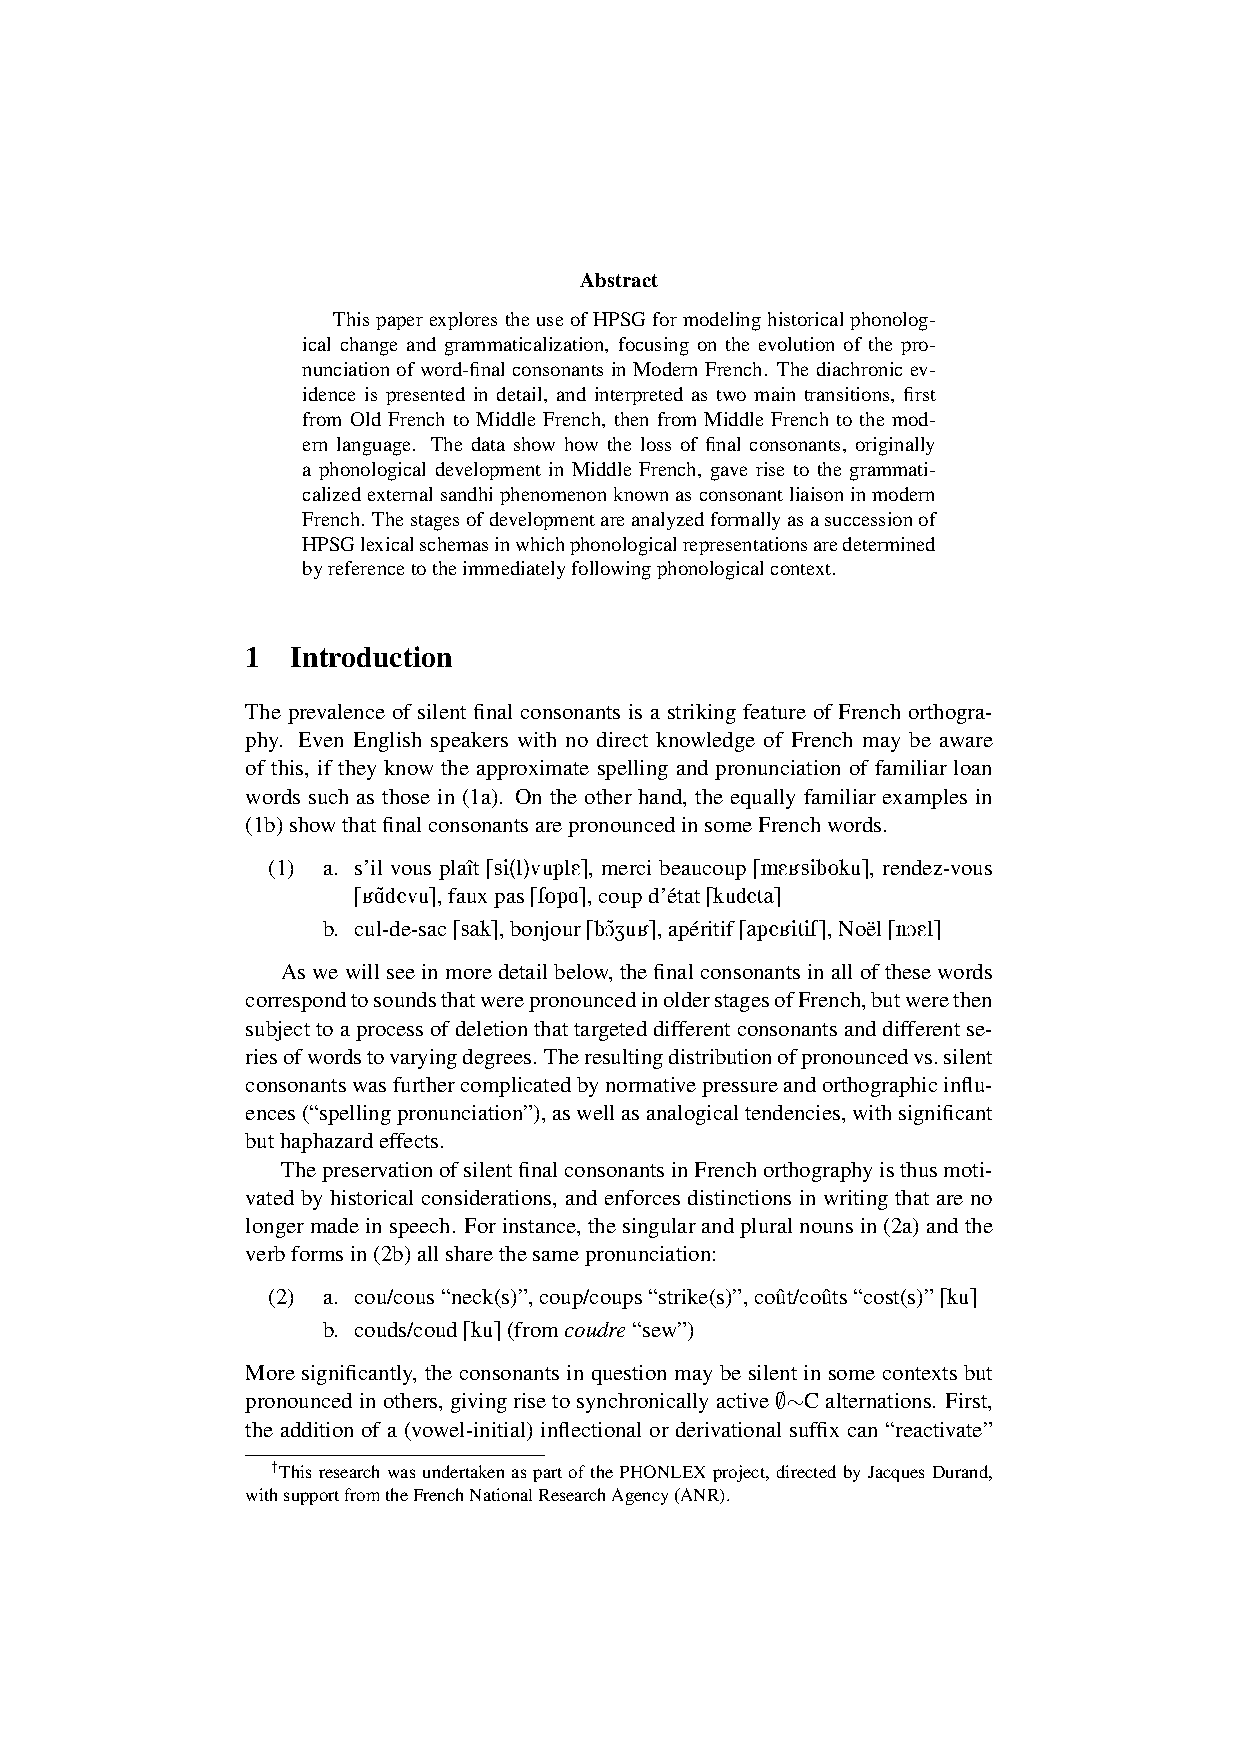
\includepdf[pages=-,pagecommand=\thispagestyle{plain}]{Includes/tseng.pdf}
        \setcounter{page}{359}
        \phantomsection
        \addcontentsline{toc}{section}{Frank Van Eynde: On the copula: from a Fregean to a Montagovian treatment}
\thispagestyle{empty}

\begin{center}
  {\huge\bfseries On the copula: from a Fregean to a Montagovian treatment\par}

  \bigskip

~\\
\begingroup
\setlength{\leftskip}{0pt plus 1fill}
\setlength{\rightskip}{0pt plus 1fill}
\setlength{\parindent}{0pt}
\setlength{\parfillskip}{0pt}
  \formatauthor{Frank Van Eynde}{\begin{tabular}{@{}c@{}}University of Leuven\end{tabular}}

\par\endgroup

  \vspace*{8ex}

  Proceedings of the 16th International Conference on\par Head-Driven Phrase Structure Grammar

  \bigskip

  Georg-August-Universit\"{a}t G{\"o}ttingen, Germany

  \medskip

  Stefan Müller (Editor)

  \medskip

  2009

  \medskip

  CSLI Publications

  \medskip

  pages 359--375

  \medskip

  \url{http://csli-publications.stanford.edu/HPSG/2009}
\end{center}
\vfill

\noindent



\vfill
\noindent
% APA Style
Van Eynde, Frank. 2009. On the copula: from a Fregean to a Montagovian treatment. In Müller, Stefan (Ed.), \emph{{Proceedings of the 16th International Conference on Head-Driven Phrase Structure Grammar, Georg-August-Universit\"{a}t G{\"o}ttingen, Germany}}, 359--375. Stanford,
CA: CSLI Publications. \hfill\href{http://creativecommons.org/licenses/by/4.0/}{\includegraphics[height=.75em]{Includes/ccby.eps}}

\newpage
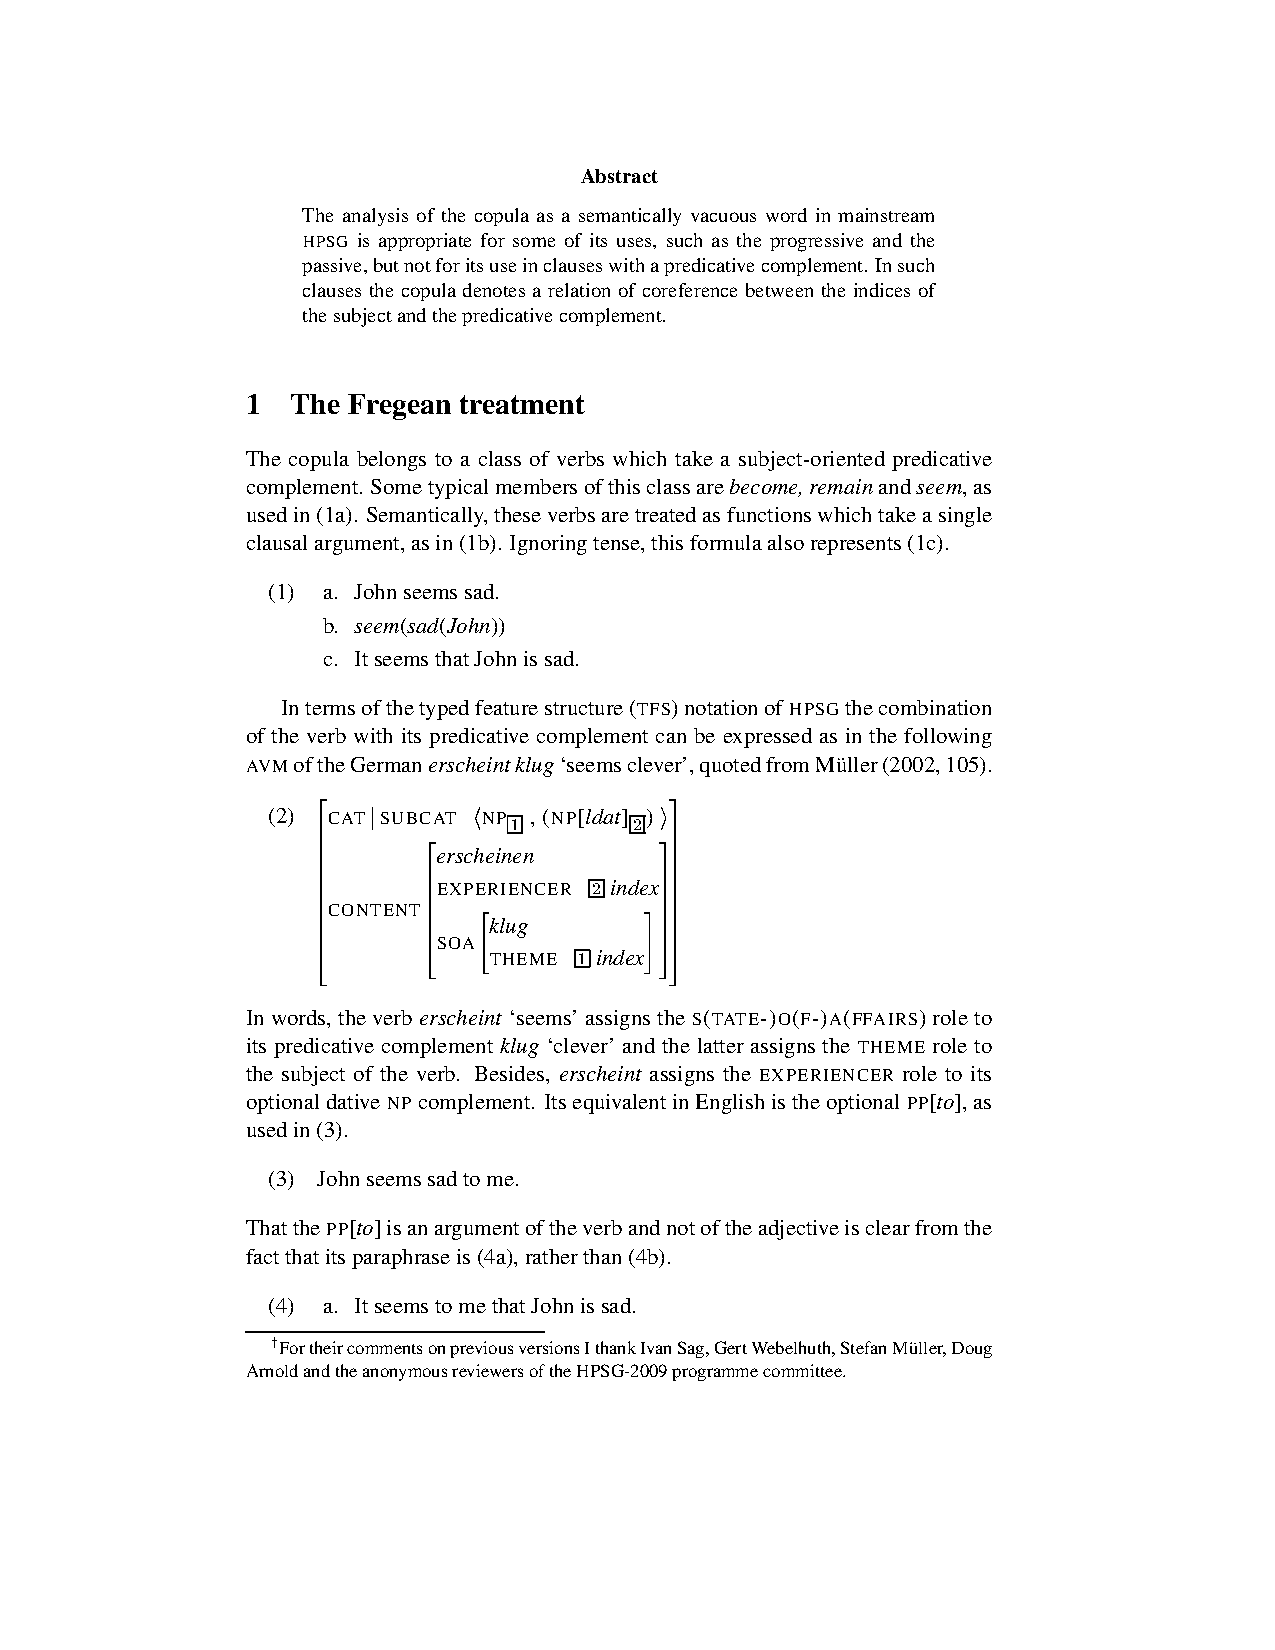
\includepdf[pages=-,pagecommand=\thispagestyle{plain}]{Includes/vaneynde.pdf}
\end{document}
